\documentclass[11pt,a4paper]{article}

\usepackage[margin=25mm]{geometry}
\usepackage[T1]{fontenc}
\usepackage[utf8]{inputenc}
\usepackage{lmodern}
\usepackage{microtype}
\usepackage{amsmath,amssymb}
\usepackage{booktabs,tabularx,longtable}
\usepackage{graphicx}
\usepackage{xcolor}
\usepackage{enumitem}
\usepackage[hidelinks]{hyperref}
\hypersetup{
  pdftitle={Verification and Validation of Canonical Fluid Flows},
  pdfauthor={Antonio Arbizzani Tonelli}
}

\graphicspath{{../../results/figures/}}
\definecolor{reportblue}{RGB}{25,82,133}
\definecolor{reportred}{RGB}{183,67,50}
\setlength{\parindent}{0pt}
\setlength{\parskip}{0.55em}
\renewcommand{\arraystretch}{1.16}
\setcounter{tocdepth}{2}
\setlist[itemize]{topsep=0.2em,itemsep=0.15em}
\pagestyle{plain}

\begin{document}

\pagenumbering{gobble}
\begin{titlepage}
  \centering
  \vspace*{22mm}
  {\color{reportblue}\rule{\linewidth}{1.4pt}}\\[9mm]
  {\LARGE\bfseries Verification and Validation of\\[2mm] Canonical Fluid Flows\par}
  \vspace{5mm}
  {\large Numerical analysis of internal flows and experimental\\
  characterisation of a circular-cylinder wake\par}
  \vspace{9mm}
  {\color{reportblue}\rule{\linewidth}{0.7pt}}\\[20mm]
  {\large Antonio Arbizzani Tonelli\par}
  \vspace{3mm}
  {\normalsize MSc in Mathematical Engineering\par}
  \vfill
  {\normalsize Academic year 2025--2026\par}
  \vspace{18mm}
\end{titlepage}

\pagenumbering{roman}
\begin{abstract}
This work presents a numerical and experimental investigation of two classes of canonical fluid-flow problems. The numerical part concerns laminar and turbulent flow in circular pipes. Mesh sensitivity, hydrodynamic development, the fully developed velocity profile, pressure losses, wall scaling, and turbulence-model performance are assessed from PHOENICS simulations. The experimental part concerns the wake and fluid forces generated by a circular cylinder in a free-surface channel. The measurement chain is first calibrated and checked for stability; particle-shadow velocimetry then resolves the mean wake and its dominant unsteadiness, while force measurements provide the mean drag and lift coefficients and an independent estimate of the shedding frequency.

The laminar calculation reproduces the Poiseuille profile with a relative $L_\infty$ error of $3.18\%$ and the analytical pressure gradient within $1.24\%$. At $Re_b=75{,}000$, the standard $k$--$\varepsilon$ model gives the closest friction factor to the experimental reference, with a relative discrepancy of $0.082\%$. The load-cell calibration is linear over the investigated range ($R^2=0.999999$), with a force RMSE of $5.72$~mN. The cylinder measurements give $\overline{C_D}=1.499$ and a force-based Strouhal number $St=0.181$; the velocity-field analysis gives $St=0.204$ at a second operating condition. The difference is interpreted in view of Reynolds number, confinement, free-surface effects, and the distinct measured quantities.
\end{abstract}

\textbf{Keywords:} CFD verification; RANS validation; pipe flow; load-cell calibration; particle-shadow velocimetry; circular-cylinder wake; uncertainty quantification.

\tableofcontents
\clearpage

\section*{Nomenclature}
\addcontentsline{toc}{section}{Nomenclature}
\begin{tabularx}{\linewidth}{@{}lX@{}}
$C_D,C_L$ & drag and lift coefficients \\
$D,R$ & pipe or cylinder diameter and radius \\
$f$ & Darcy friction factor \\
$f_s$ & dominant shedding frequency \\
$k,\varepsilon$ & turbulent kinetic energy and dissipation rate \\
$Re$ & Reynolds number \\
$St=f_sD/U_b$ & Strouhal number \\
$U_b,W_b$ & bulk velocity in the channel and pipe \\
$u_\tau$ & friction velocity \\
$y^+,W^+$ & inner-scaled wall distance and axial velocity \\
$\rho,\mu,\nu$ & density, dynamic viscosity, and kinematic viscosity
\end{tabularx}

\clearpage
\pagenumbering{arabic}
\section{Scope and validation strategy}

The study combines numerical and experimental evidence for two canonical fluid-mechanics problems. Pipe flow provides analytical relations and established friction laws for the assessment of CFD calculations. The circular cylinder provides a separated, unsteady flow for which local velocity measurements and integral force measurements offer complementary descriptions.

The work is organised as an evidence chain rather than as a sequence of independent exercises:
\begin{enumerate}
    \item establish numerical resolution through controlled grid refinements;
    \item verify the laminar calculation against the Poiseuille solution and the analytical pressure gradient;
    \item validate turbulent closures against measured profiles and an experimental friction factor;
    \item calibrate the force transducer and quantify the residual measurement error;
    \item identify the cylinder wake from velocity fields and force records;
    \item compare the independent shedding-frequency estimates and retain the limitations of the comparison.
\end{enumerate}

Verification is used here in the strict sense of assessing whether the numerical formulation and post-processing reproduce a known solution. Validation instead assesses agreement with measurements. Grid sensitivity is reported separately from both: convergence between successive grids is necessary, but it does not demonstrate physical accuracy by itself \cite{celik2008}.

The pipe-flow and cylinder datasets do not constitute a single coupled experiment. The geometries and operating conditions are different, and the two cylinder acquisitions were performed at different flow rates and water depths. Their connection lies in the common use of reference quantities and quantitative error measures.

\subsection{Objectives}

The analysis considers:
\begin{itemize}
    \item mesh-sensitivity metrics for laminar and turbulent pipe flows;
    \item hydrodynamic entry lengths, developed profiles, and pressure-loss estimates;
    \item a comparison of four $k$--$\varepsilon$ configurations at $Re_b=75{,}000$;
    \item calibration coefficients, stability times, and force residuals for sixteen loads;
    \item mean wake fields, velocity-deficit profiles, vorticity phases, and a probe spectrum;
    \item mean force coefficients, a lift spectrum, and a first-order uncertainty budget.
\end{itemize}

\section{Numerical methodology}

\subsection{Flow configurations}

The internal-flow calculations were performed in an axisymmetric representation of a circular pipe. The laminar case uses $D=0.15$~m, $W_b=0.45$~m/s, $\rho=910$~kg/m$^3$, and $\nu=3.5\times10^{-4}$~m$^2$/s, giving
\begin{equation}
Re_b=\frac{W_bD}{\nu}=192.9.
\end{equation}
The turbulent case uses $D=0.10$~m, $W_b=0.75$~m/s, and $\nu=10^{-6}$~m$^2$/s, hence $Re_b=75{,}000$. The simulations were performed with PHOENICS. The calculated fields include velocity, pressure, wall stress, eddy viscosity, turbulent kinetic energy, and dissipation rate.

Four turbulent configurations are retained: standard $k$--$\varepsilon$, RNG $k$--$\varepsilon$, realisable $k$--$\varepsilon$, and a low-Reynolds-number $k$--$\varepsilon$ treatment. The comparison is specific to the implemented grids and wall treatments; it is not intended as a general ranking of the closures \cite{launder1974}.

\subsection{Grid-sensitivity procedure}

Three refinement paths are considered for each regime. Radial refinement changes the number of cells across the radius, axial refinement changes the streamwise resolution, and combined refinement changes both. Profiles are extracted at $z\simeq0.8L$ for the radial and combined sequences. Axial refinement is assessed from the pressure distribution at approximately half radius.

For successive grids $i$ and $i+1$, the reported indicator is
\begin{equation}
\epsilon_{i,i+1}=\frac{\left\|\phi_i^{\,\mathrm{int}}-\phi_{i+1}\right\|_\infty}
{\left\|\phi_{i+1}\right\|_\infty},
\end{equation}
where the coarser result is linearly interpolated to the finer coordinates. This is a transparent pairwise sensitivity measure. It is not a formal Grid Convergence Index because the available grids do not define a uniform refinement ratio for all directions.

\subsection{Developed-flow and pressure-loss estimators}

The last interior velocity profile is used as the developed reference. At each axial station,
\begin{equation}
\epsilon_p(z)=\frac{\|W(r,z)-W_{\mathrm{ref}}(r)\|_\infty}
{\|W_{\mathrm{ref}}(r)\|_\infty}.
\end{equation}
The numerical development length is the first station at which $\epsilon_p\leq10^{-3}$. This stringent threshold should be read as an operational definition tied to the sampled grid.

For the laminar case, the area-weighted mean pressure is
\begin{equation}
\overline{p}(z)=\frac{2}{R^2}\int_0^R p(r,z)r\,\mathrm{d}r.
\end{equation}
A least-squares line fitted to the last developed stations gives the numerical pressure gradient. The reference values are the Poiseuille profile and pressure gradient,
\begin{equation}
\frac{W(r)}{W_b}=2\left[1-\left(\frac{r}{R}\right)^2\right],
\qquad
\frac{\mathrm{d}p}{\mathrm{d}z}=-\frac{32\mu W_b}{D^2}.
\end{equation}

For the turbulent case, the Darcy friction factor is obtained from the computed wall stress,
\begin{equation}
f=\frac{8\tau_w}{\rho W_b^2},
\end{equation}
and compared with the experimental value, the smooth-pipe Prandtl relation, and the Haaland expression \cite{haaland1983}. Velocity-profile error is measured by the RMSE after interpolating the CFD profile to the experimental radial coordinates.

\section{Laminar CFD verification}

\subsection{Grid sensitivity}

Figure~\ref{fig:laminar-grid} reports the three refinement paths. The velocity profiles and pressure distributions approach a stable result without changes in shape or non-physical oscillations. The relative $L_\infty$ changes are summarised in Table~\ref{tab:grid-errors}. Radial sensitivity decreases from $2.36\%$ to $0.52\%$, while axial sensitivity decreases from $0.41\%$ to $0.23\%$. The combined medium-to-fine difference remains below $1\%$.

\begin{figure}[htbp]
    \centering
    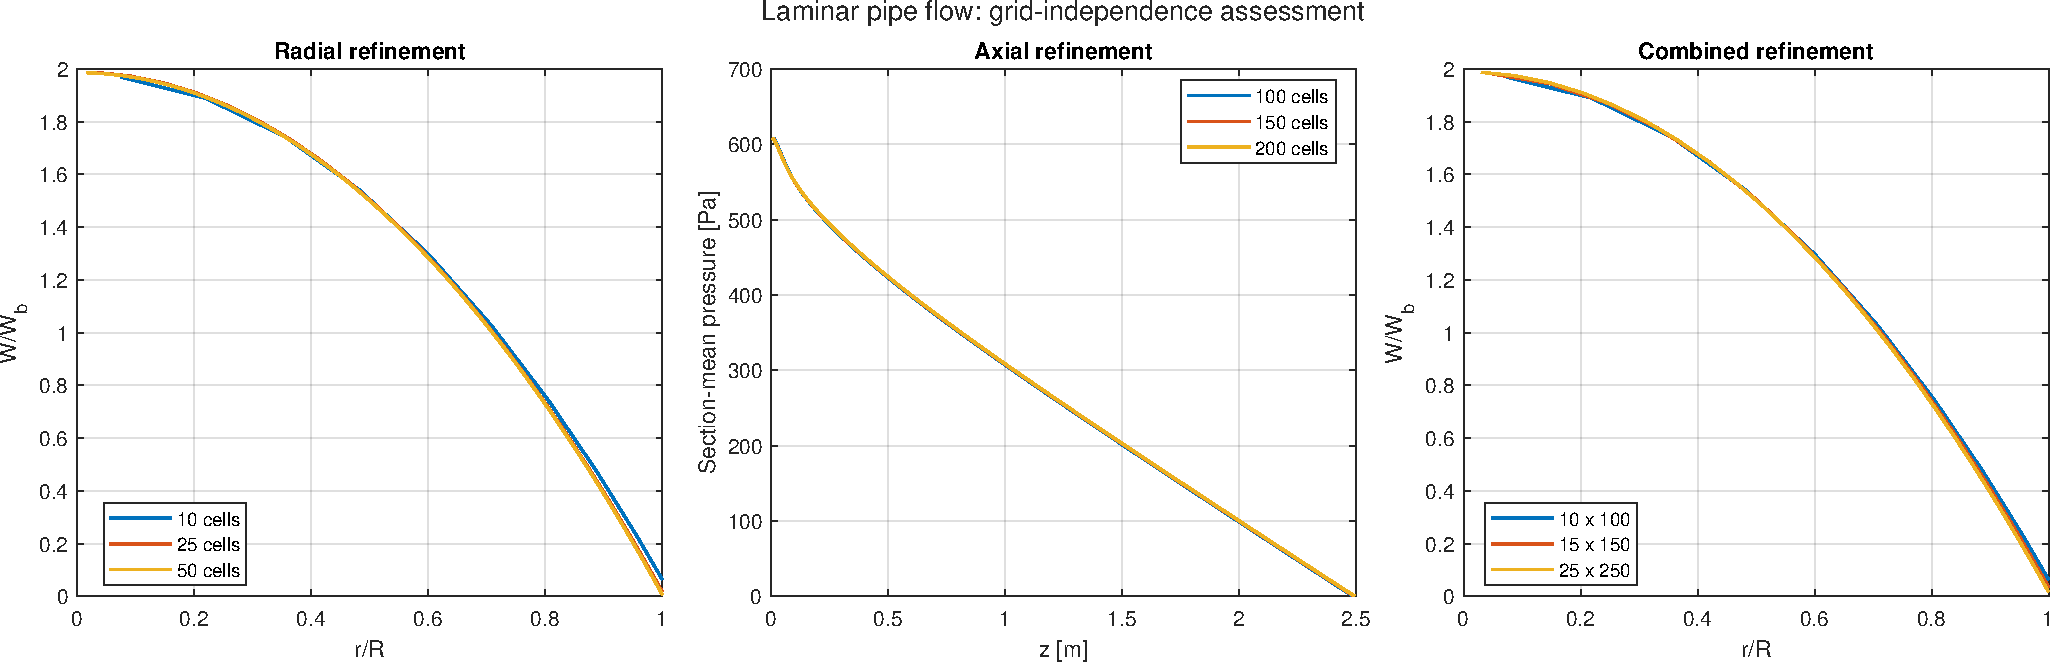
\includegraphics[width=\linewidth]{laminar_grid_independence.pdf}
    \caption{Laminar-flow grid study: radial velocity, axial pressure, and combined refinement.}
    \label{fig:laminar-grid}
\end{figure}

\begin{table}[htbp]
\centering
\caption{Successive-grid relative $L_\infty$ differences.}
\label{tab:grid-errors}
\begin{tabular}{llrr}
\toprule
Regime & Direction & coarse--medium [\%] & medium--fine [\%] \\
\midrule
Laminar & radial & 2.359 & 0.521 \\
Laminar & axial & 0.412 & 0.225 \\
Laminar & combined & 1.438 & 0.925 \\
Turbulent & radial & 0.842 & 0.242 \\
Turbulent & axial & 0.260 & 0.132 \\
Turbulent & combined & 0.625 & 0.366 \\
\bottomrule
\end{tabular}
\end{table}

The finest solutions are retained for the following comparisons. The table also anticipates the turbulent results discussed in Section~\ref{sec:turbulent-validation}. Since the errors are defined from different observables for radial and axial refinements, magnitudes should only be compared within the same direction.

\subsection{Hydrodynamic development}

The usual laminar estimate $L_e=0.0575ReD$ gives $1.663$~m. The $0.1\%$ profile criterion gives a numerical development length of $2.113$~m. Figure~\ref{fig:laminar-development} shows that the centreline velocity tends towards $2W_b$, while the complete profile approaches the final reference monotonically.

\begin{figure}[htbp]
    \centering
    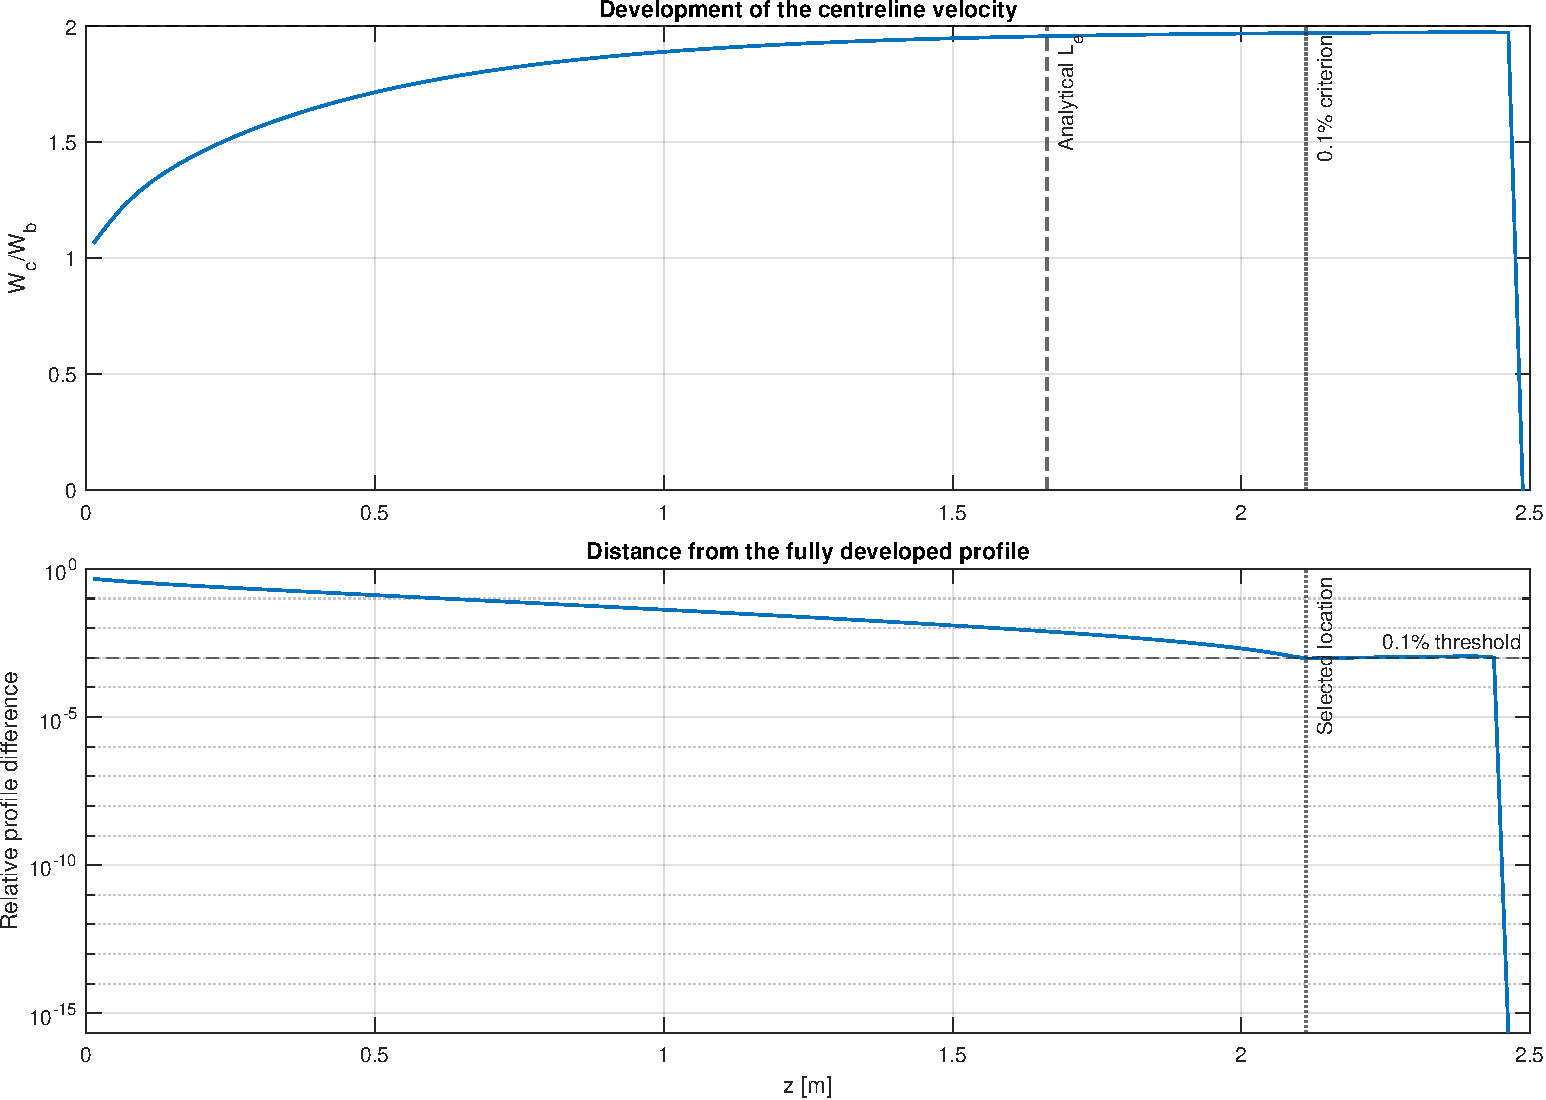
\includegraphics[width=0.90\linewidth]{laminar_flow_development.pdf}
    \caption{Laminar development based on the centreline velocity and the distance from the final profile.}
    \label{fig:laminar-development}
\end{figure}

The numerical value is $27\%$ larger than the correlation estimate. This discrepancy is compatible with the strict full-profile threshold, the discrete axial sampling, and the fact that engineering entry-length correlations generally rely on less restrictive local criteria. The important result is not exact equality between the two definitions, but the correct asymptotic state and a documented selection rule.

\subsection{Fully developed profile}

The bulk velocity reconstructed from the final CFD profile is $0.4523$~m/s, within $0.51\%$ of the imposed value. Figure~\ref{fig:laminar-profile} compares the normalised solution with the analytical parabola. The relative $L_\infty$ profile error is $3.18\%$. The largest visible discrepancy is confined to the outer part of the profile, where spatial resolution and the discrete wall treatment have the strongest effect.

\begin{figure}[htbp]
    \centering
    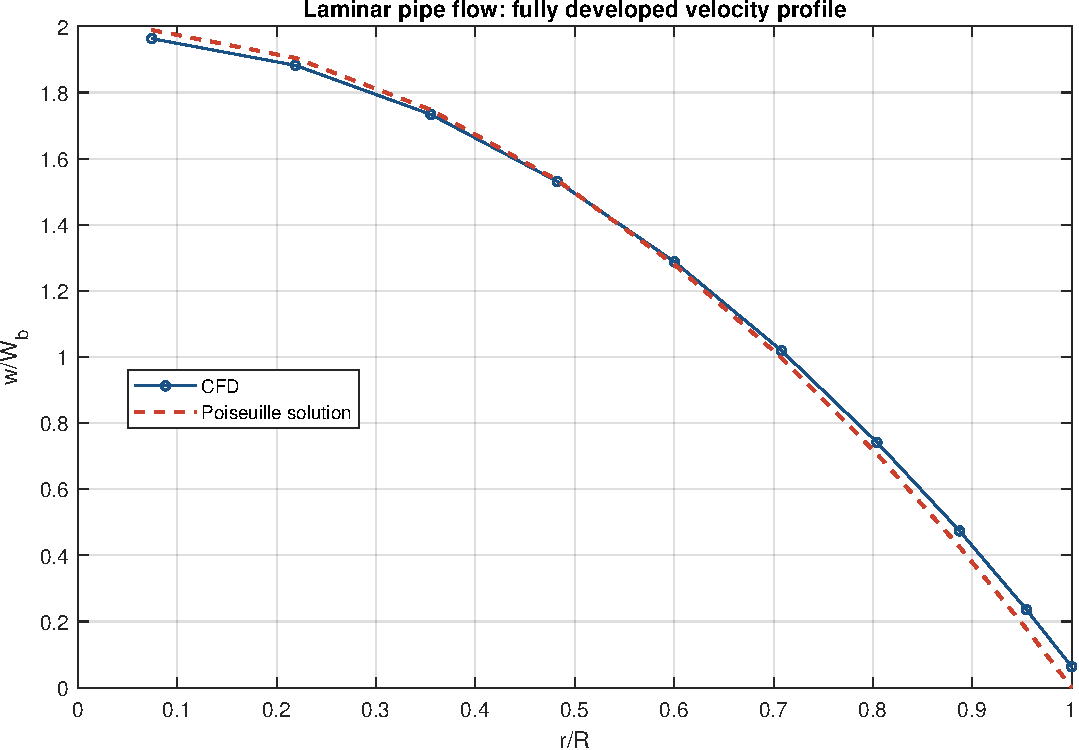
\includegraphics[width=0.72\linewidth]{laminar_pipe_verification.pdf}
    \caption{Fully developed laminar velocity profile against the Poiseuille solution.}
    \label{fig:laminar-profile}
\end{figure}

\subsection{Pressure gradient}

The analytical gradient is $-203.84$~Pa/m. Linear regression over the last developed stations gives $-201.32$~Pa/m, corresponding to a relative error of $1.24\%$. Figure~\ref{fig:laminar-pressure} also confirms that the pressure becomes linear once the inlet development is complete.

\begin{figure}[htbp]
    \centering
    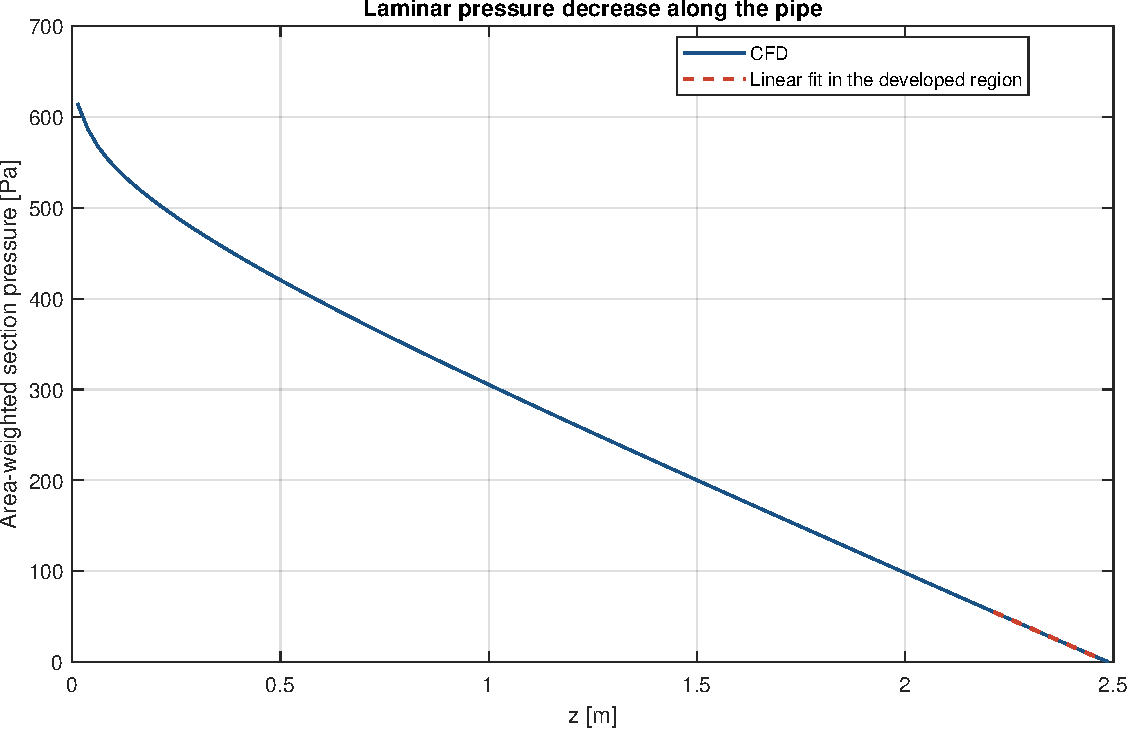
\includegraphics[width=0.76\linewidth]{laminar_pressure_gradient.pdf}
    \caption{Area-weighted pressure and linear fit in the developed region.}
    \label{fig:laminar-pressure}
\end{figure}

The agreement of both profile shape and pressure loss is more informative than agreement in either quantity alone. The first checks the velocity field; the second checks the integral momentum balance and the wall shear implied by the solution.

\section{Turbulent CFD validation}\label{sec:turbulent-validation}

\subsection{Grid sensitivity and streamwise development}

The turbulent grid study in Figure~\ref{fig:turbulent-grid} gives smaller pairwise differences than the laminar study. Medium-to-fine changes are $0.24\%$, $0.13\%$, and $0.37\%$ for radial, axial, and combined refinement, respectively. These values support the use of the retained grids for model comparison, while remaining conditional on the chosen observables.

\begin{figure}[htbp]
    \centering
    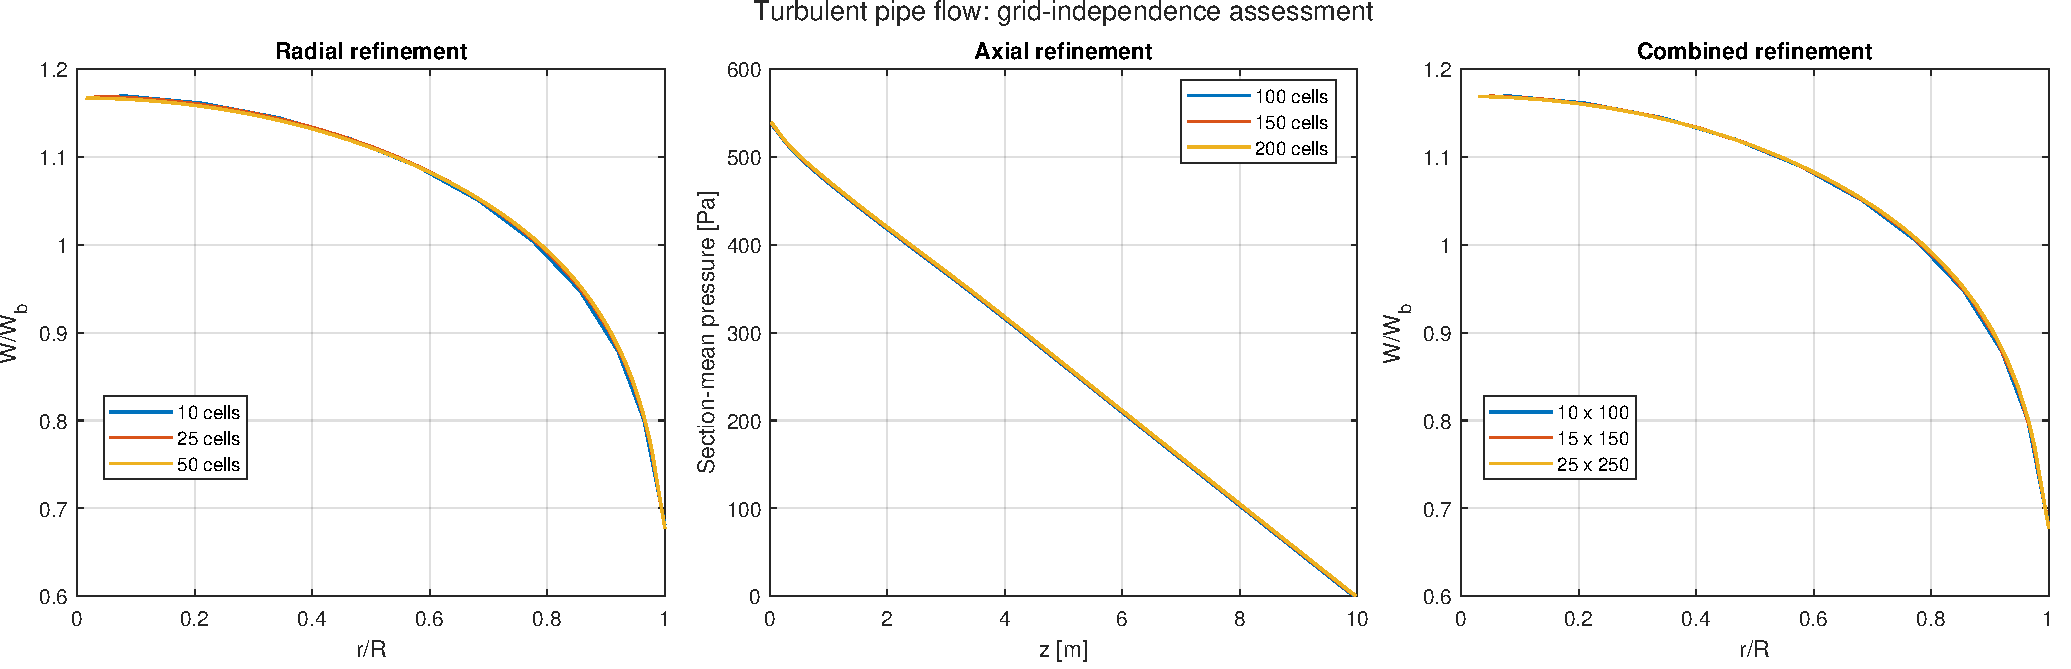
\includegraphics[width=\linewidth]{turbulent_grid_independence.pdf}
    \caption{Turbulent-flow grid study: radial velocity, axial pressure, and combined refinement.}
    \label{fig:turbulent-grid}
\end{figure}

The correlation $L_e=1.359DRe^{1/4}$ gives $2.249$~m. The full-profile $0.1\%$ criterion is first satisfied at $z=9.85$~m, close to the final interior station. Figure~\ref{fig:turbulent-development} explains the difference: the centreline velocity reaches an approximately stable level earlier, whereas the full radial profile continues to change weakly. The result illustrates the sensitivity of a turbulent entry length to its definition.

\begin{figure}[htbp]
    \centering
    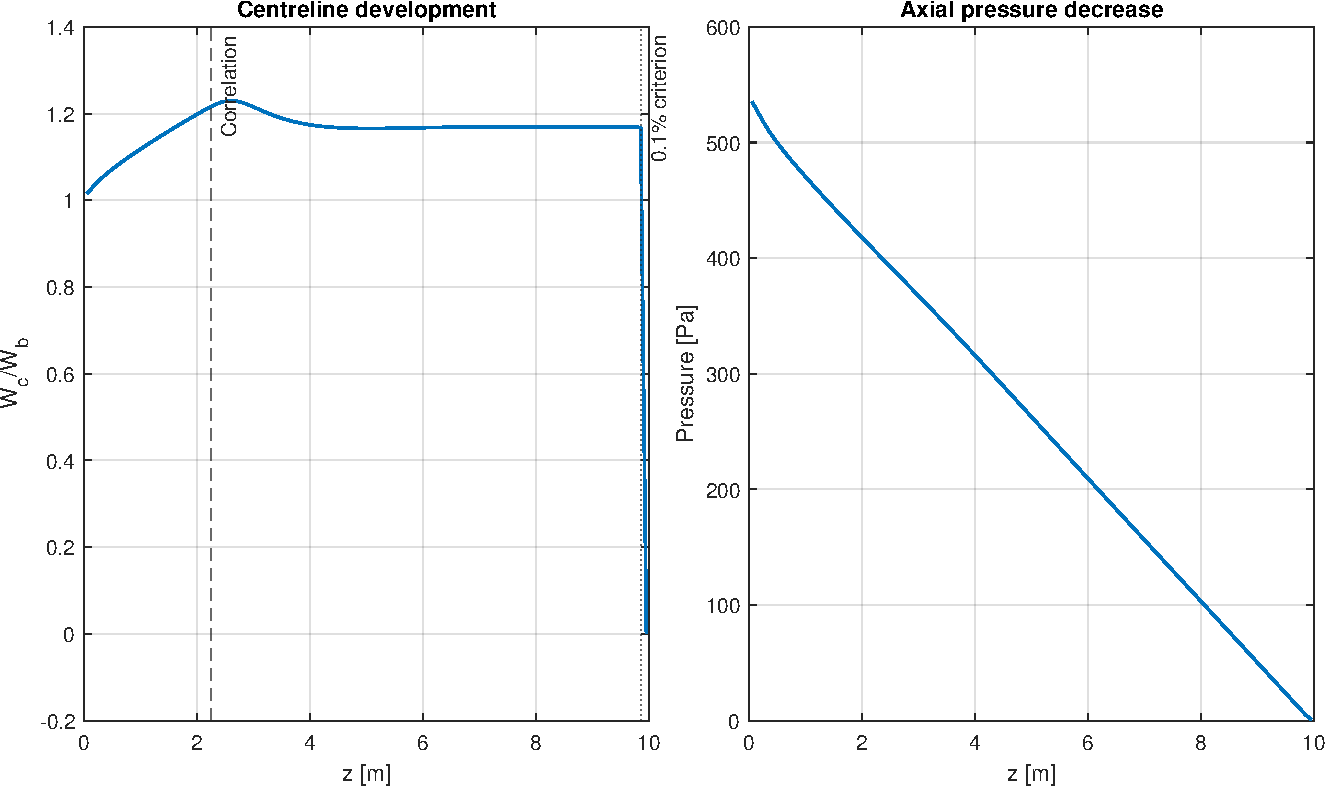
\includegraphics[width=0.84\linewidth]{turbulent_flow_development.pdf}
    \caption{Centreline-velocity development and axial pressure decrease for the standard $k$--$\varepsilon$ case.}
    \label{fig:turbulent-development}
\end{figure}

\subsection{Resolved mean and turbulence fields}

Figure~\ref{fig:turbulent-structure} collects the fully developed mean velocity, eddy-viscosity ratio, turbulent kinetic energy, and dissipation rate. The mean profile is flatter than the laminar parabola. Turbulent quantities increase towards the wall region, consistent with shear production, while the centreline symmetry is retained.

\begin{figure}[htbp]
    \centering
    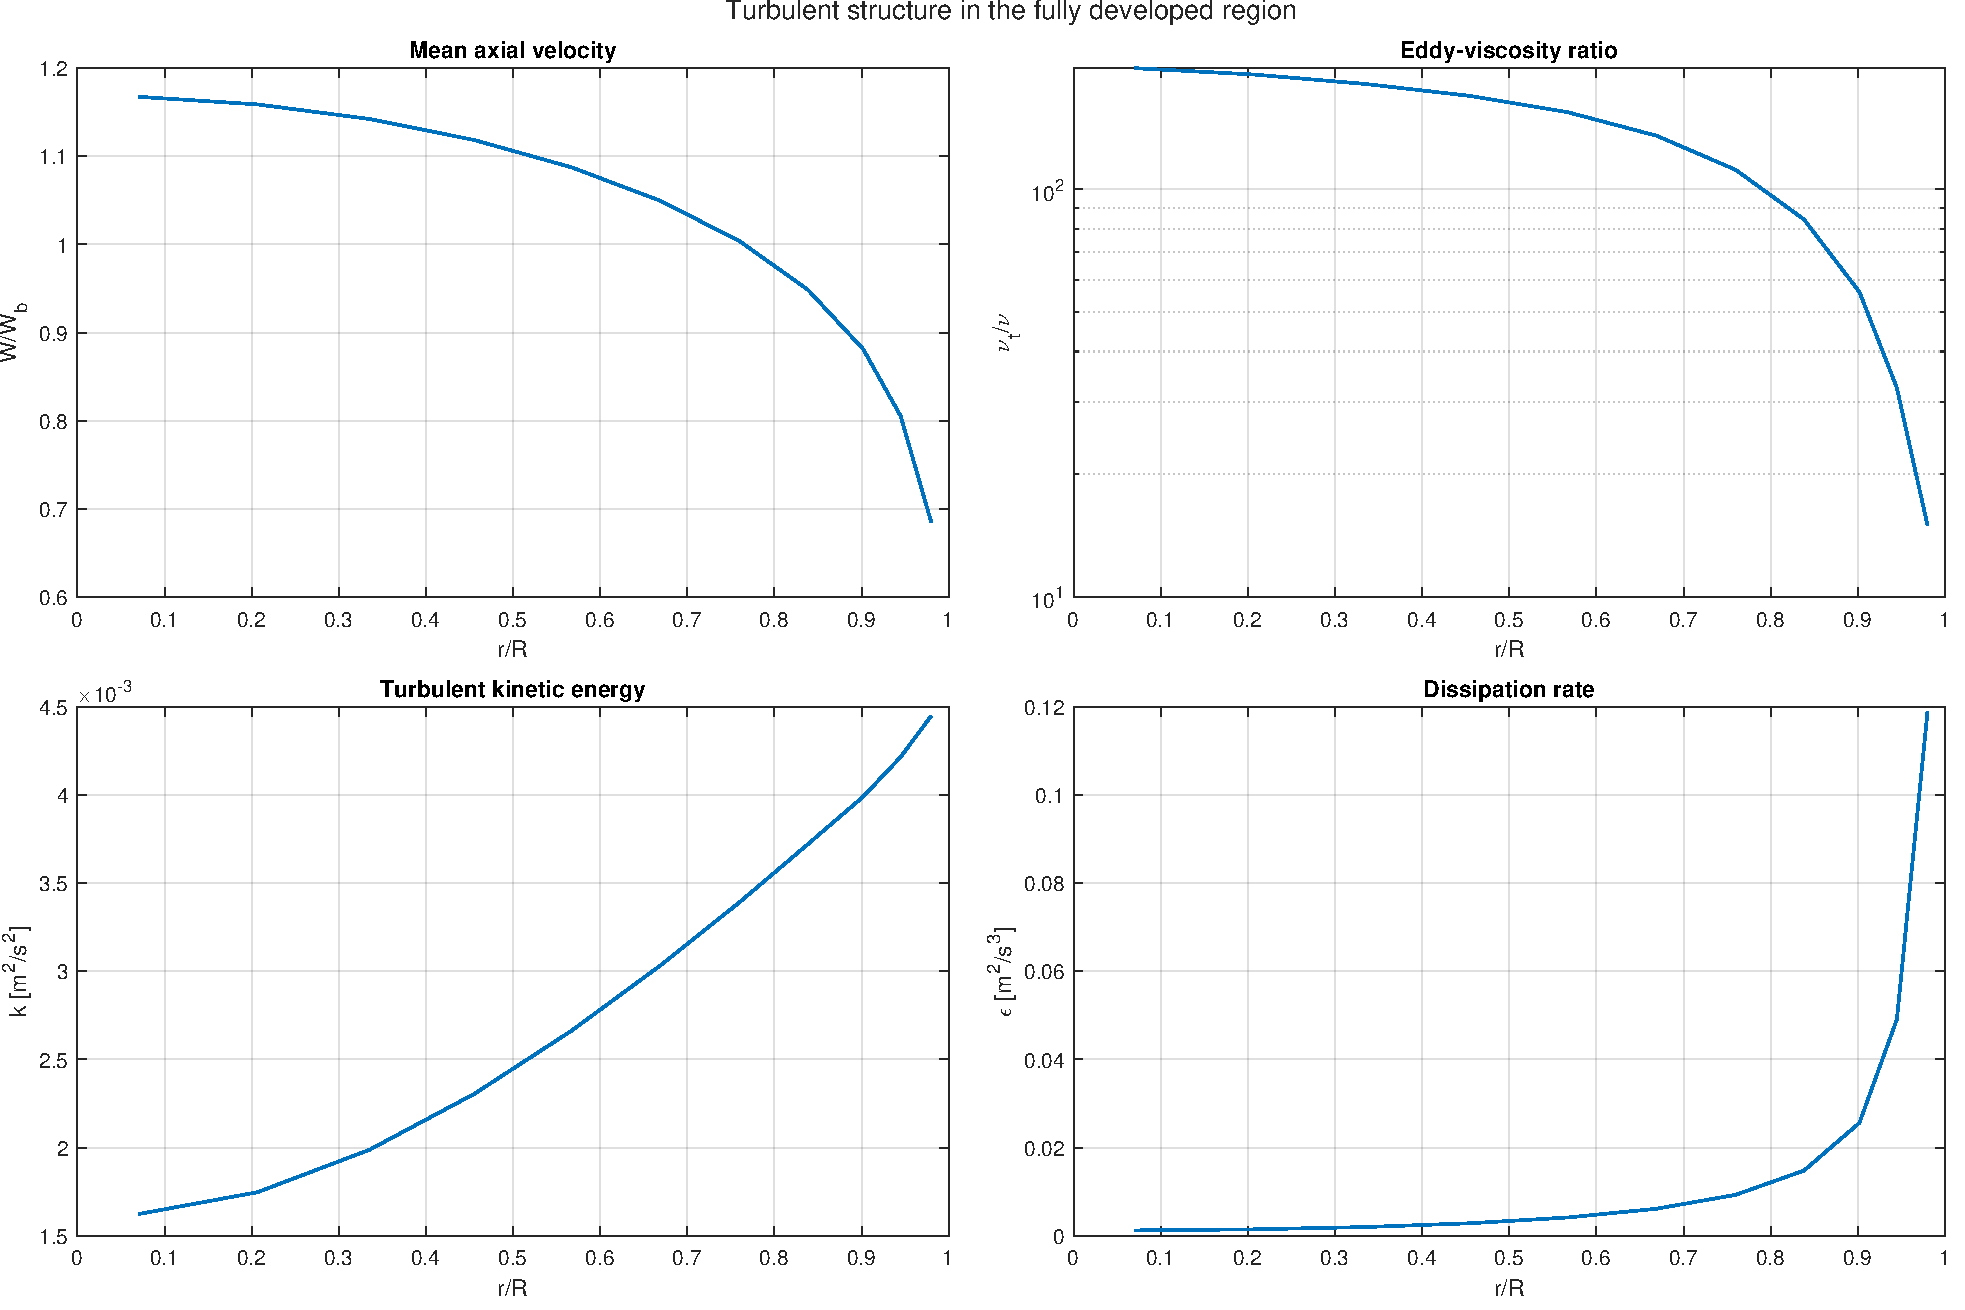
\includegraphics[width=0.94\linewidth]{turbulent_structure_profiles.pdf}
    \caption{Radial structure of the standard $k$--$\varepsilon$ solution in the developed region.}
    \label{fig:turbulent-structure}
\end{figure}

The wall stress gives $u_\tau=0.03654$~m/s. Figure~\ref{fig:wall-scaling} compares the computed inner-scaled velocity with the viscous and logarithmic reference laws. The maximum plotted $y^+$ is approximately $1699$ because it corresponds to the distance from the wall to the pipe axis; it is not the first-cell wall coordinate. The profile crosses the expected logarithmic range but the near-wall assessment remains limited by the available cell-centre sampling.

\begin{figure}[htbp]
    \centering
    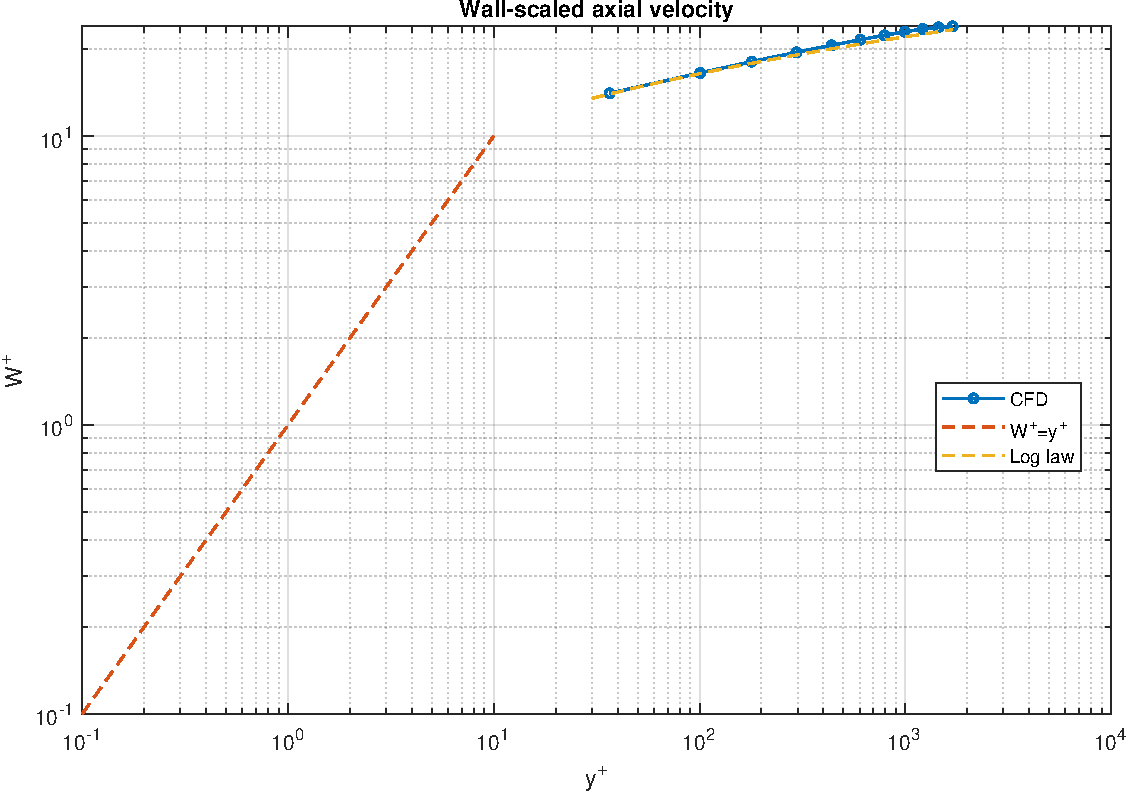
\includegraphics[width=0.70\linewidth]{turbulent_wall_scaling.pdf}
    \caption{Wall-scaled axial velocity for the standard $k$--$\varepsilon$ case.}
    \label{fig:wall-scaling}
\end{figure}

\subsection{Model comparison}

Figure~\ref{fig:turbulent-profiles} compares the four numerical profiles with two experimental series. All closures reproduce the main shape. The standard model gives the lowest normalised profile RMSE, $0.0158$, followed by RNG ($0.0166$), realisable ($0.0195$), and low-Re ($0.0214$).

\begin{figure}[htbp]
    \centering
    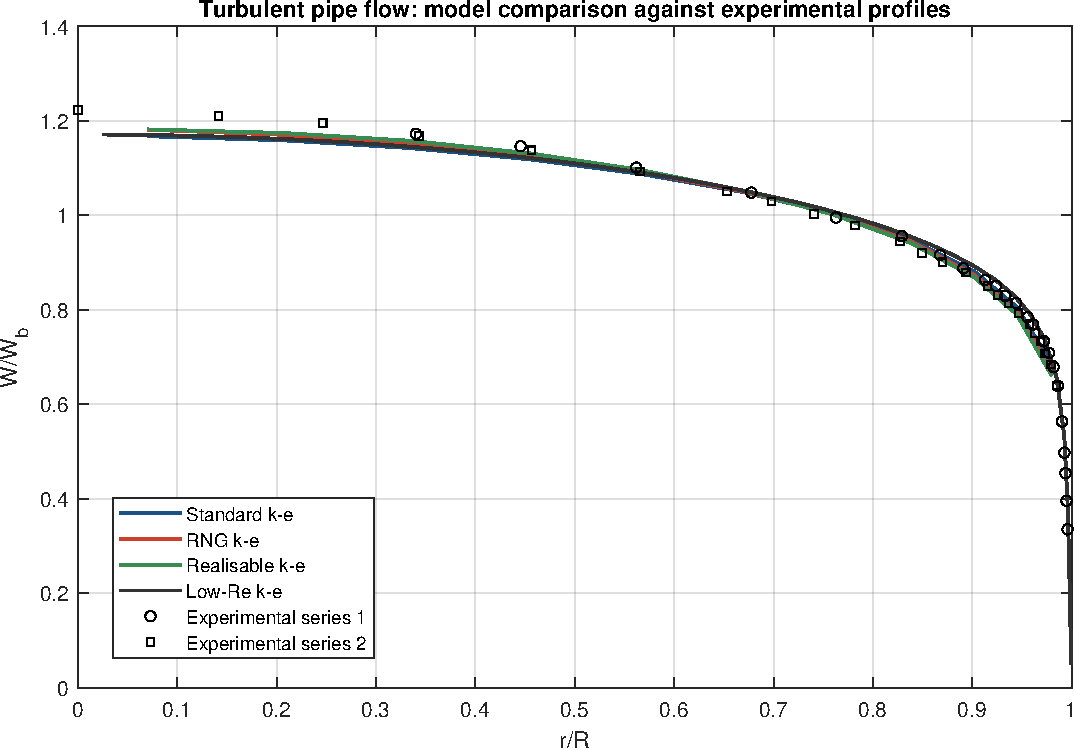
\includegraphics[width=0.76\linewidth]{turbulent_pipe_validation.pdf}
    \caption{Turbulent velocity profiles and experimental measurements at $Re_b=75{,}000$.}
    \label{fig:turbulent-profiles}
\end{figure}

\begin{table}[htbp]
\centering
\caption{Turbulence-model validation metrics.}
\label{tab:turbulent-models}
\begin{tabular}{lrrr}
\toprule
Model & $f$ & $|f-f_{\mathrm{exp}}|/f_{\mathrm{exp}}$ [\%] & Profile RMSE \\
\midrule
Standard $k$--$\varepsilon$ & 0.018984 & 0.082 & 0.01584 \\
RNG $k$--$\varepsilon$ & 0.018403 & 3.143 & 0.01659 \\
Realisable $k$--$\varepsilon$ & 0.017853 & 6.035 & 0.01948 \\
Low-Re $k$--$\varepsilon$ & 0.021688 & 14.148 & 0.02144 \\
\bottomrule
\end{tabular}
\end{table}

The experimental Darcy factor is $0.0190$. The smooth-pipe Prandtl and Haaland values are $0.01912$ and $0.01895$, respectively. Figure~\ref{fig:friction-comparison} shows that the standard model is also closest to all three references. The low-Re configuration overpredicts wall friction in the present implementation; this is consistent with a mismatch between a wall-resolving formulation and the available near-wall resolution rather than with an intrinsic failure of the closure.

\subsection{Low-Reynolds-number resolution sensitivity}

The low-Reynolds-number case was examined separately because its friction-factor discrepancy is larger than that of the other closures. Four radial meshes, with $N_y=35$, 45, 60, and 75 cells, were compared using the developed-region velocity profile at $z/L\simeq0.8$. The successive relative $L_\infty$ changes are $1.10\%$, $0.55\%$, and $3.15\%$. The final change is not smaller than the preceding one; the sequence therefore does not establish monotonic convergence or grid independence for this observable.

\begin{figure}[htbp]
    \centering
    \includegraphics[width=0.82\linewidth]{low_re_grid_sensitivity.pdf}
    \caption{Developed-region low-Reynolds-number profiles for four radial meshes.}
    \label{fig:low-re-grid}
\end{figure}

The three solver exports available on the $N_y=45$ mesh permit a complementary iteration-sensitivity check. From 500 to 750 iterations, the relative $L_\infty$ changes are $0.96\%$ in axial velocity, $1.89\%$ in pressure, $4.58\%$ in turbulent kinetic energy, $6.54\%$ in dissipation rate, and $12.30\%$ in eddy viscosity. From 750 to 1000 iterations, they decrease to $0.23\%$, $0.33\%$, $1.19\%$, $3.03\%$, and $4.05\%$, respectively. The mean-flow fields change less than the turbulence quantities at the final iteration interval, but the latter have not reached a demonstrated asymptote.

\begin{figure}[htbp]
    \centering
    \includegraphics[width=0.84\linewidth]{low_re_iteration_sensitivity.pdf}
    \caption{Relative field changes between successive low-Reynolds-number solver exports.}
    \label{fig:low-re-iterations}
\end{figure}

An additional comparison varies the radial-spacing exponent while keeping the nominal radial cell count fixed at 11. The profile changes are $0.66\%$ between $p=-1.5$ and $p=-1.8$, and $0.37\%$ between $p=-1.8$ and $p=-2.0$. This supports limited sensitivity to the tested spacing choices, but it does not resolve the non-monotonic cell-count study or the remaining turbulence-field iteration changes.

\begin{figure}[htbp]
    \centering
    \includegraphics[width=0.78\linewidth]{power_y_stretching_sensitivity.pdf}
    \caption{Low-Reynolds-number profiles for three radial-spacing exponents at fixed nominal cell count.}
    \label{fig:low-re-spacing}
\end{figure}

\begin{figure}[htbp]
    \centering
    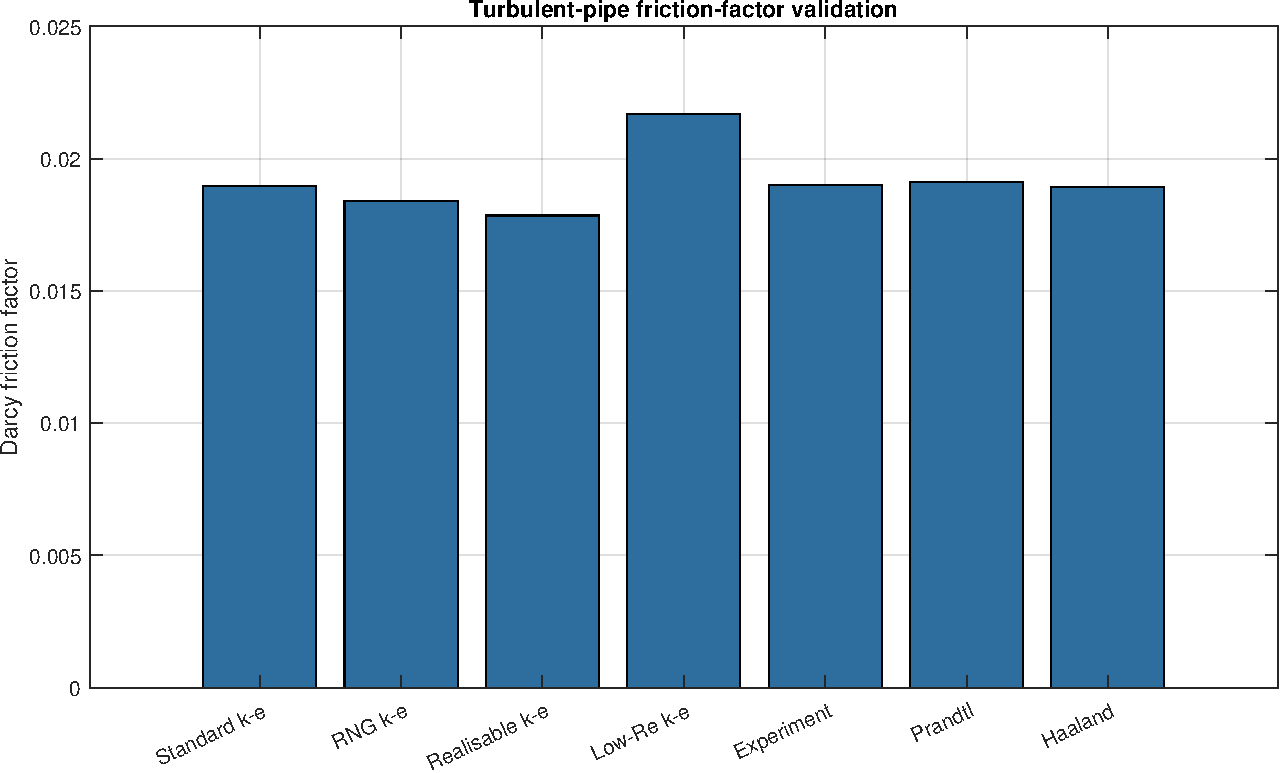
\includegraphics[width=0.80\linewidth]{turbulent_friction_factor_comparison.pdf}
    \caption{Darcy friction factors from the RANS solutions, experiment, and smooth-pipe correlations.}
    \label{fig:friction-comparison}
\end{figure}

\section{Experimental methodology}

\subsection{Load-cell calibration}

Sixteen static reference loads span approximately $-10.5$ to $13.8$~N and include both loading directions. Each voltage acquisition is sampled at 100~Hz. The steady response is defined as the mean of the final $30\%$ of the record. A linear transfer relation is fitted in the voltage domain,
\begin{equation}
V=S F+V_0,
\end{equation}
where $S$ is the sensitivity and $V_0$ the zero-load offset. Residuals are then mapped back to force units.

Stability is assessed from the cumulative mean. The signal is classified as stable when the cumulative mean remains within $2\%$ of a normalisation scale based on the final level and the signal range. This metric is intentionally operational: it detects the time after which the estimate no longer leaves the acceptance band, but it is not a dynamic model of the transducer.

\subsection{Particle-shadow velocimetry}

The wake dataset contains 1499 displacement fields on a $23\times30$ grid sampled at 50~Hz. Pixel displacements are converted to velocity using the spatial resolution of 3040~px/m. Coordinates are translated to the cylinder reference frame and normalised by $D=0.06$~m. For a channel width of $0.50$~m, water depth of $0.42$~m, and flow rate of 35~L/s,
\begin{equation}
U_b=0.1667\ \mathrm{m/s}, \qquad Re_D=\frac{U_bD}{\nu}=9.98\times10^3.
\end{equation}

Invalid vectors are omitted in the time average. The cylinder interior is masked before plotting. The spectral probe is selected as the valid grid point nearest to $(x/D,y/D)=(0.25,0)$; missing samples are linearly interpolated in time. The dominant peak is searched between 0.2 and 10~Hz to exclude the mean component and high-frequency noise. Four vorticity snapshots separated by one quarter of the identified period provide a phase-resolved representation of the shedding cycle. These phases originate from a moving-average filtered sequence and should be interpreted qualitatively rather than as an ensemble phase average \cite{raffel2018}.

\subsection{Force measurements}

The force experiment uses a channel width of $0.50$~m, water depth of $0.45$~m, flow rate of 75~L/s, cylinder diameter of $0.06$~m, and instrumented span of $0.185$~m. The bulk velocity is $U_b=0.3333$~m/s. A still-water record provides the vertical buoyancy offset. After correction,
\begin{equation}
C_D=\frac{F_D}{\tfrac12\rho U_b^2DL}, \qquad
C_L=\frac{F_L}{\tfrac12\rho U_b^2DL}.
\end{equation}

The one-sided Fourier amplitude is obtained after removing the signal mean. The dominant non-zero lift peak gives $f_s$ and $St=f_sD/U_b$. The acquisition is sampled at 200~Hz.

\subsection{First-order uncertainty propagation}

Standard uncertainties assigned to the measurement chain are 0.045~N for drag, 0.025~N for each vertical-force contribution, 1~mm for depth and channel width, 0.05~mm for cylinder diameter, and 1~mm for span. Flow-rate uncertainty combines a $0.5\%$ relative contribution with the effect of a 1~mm head uncertainty in the 0.20~m meter pipe. Independent contributions are propagated with a root-sum-of-squares approximation. The resulting values quantify the stated instrument model; they do not include model-form errors due to free-surface deformation, blockage, end effects, or imperfect alignment.

\section{Measurement-chain calibration}

\subsection{Static transfer function}

The fitted sensitivity is $S=-4.07807\times10^{-4}$~V/N and the offset is $V_0=-2.86673\times10^{-5}$~V. The sign follows the electrical convention of the acquisition system. Figure~\ref{fig:load-calibration} shows no evident change in slope between positive and negative loads.

\begin{figure}[htbp]
    \centering
    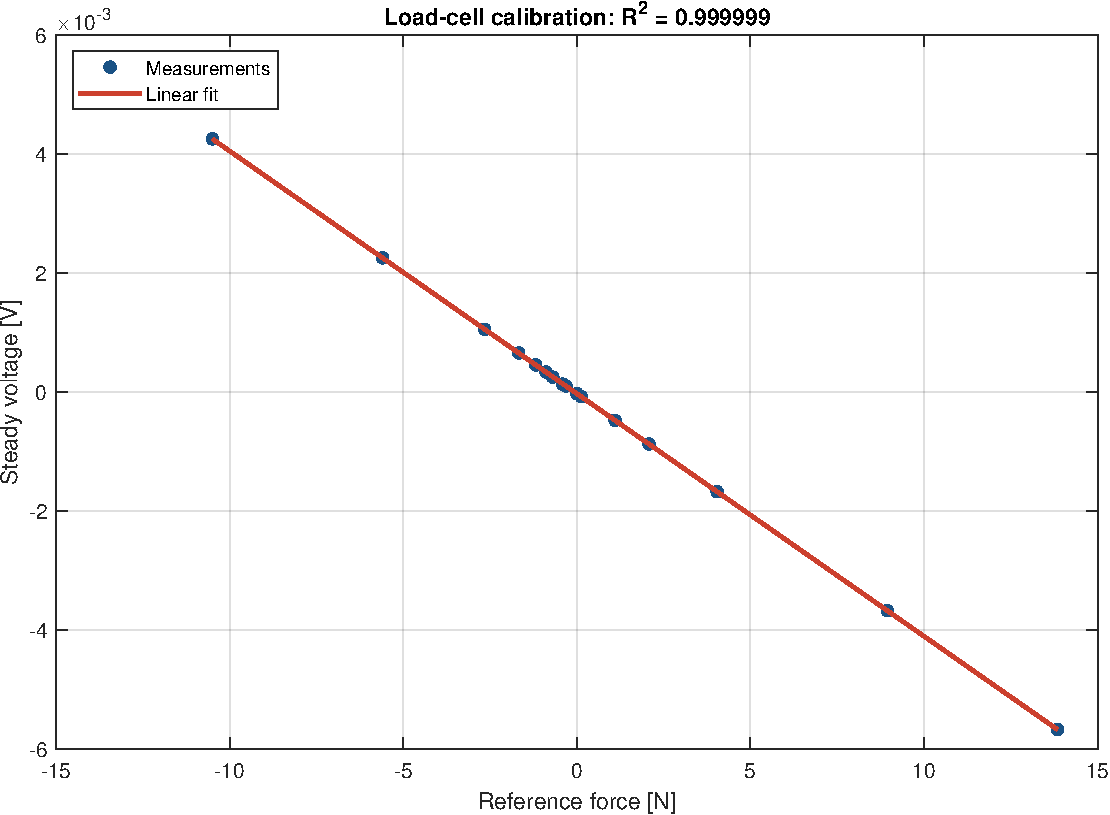
\includegraphics[width=0.74\linewidth]{load_cell_calibration.pdf}
    \caption{Static load-cell calibration from sixteen reference loads.}
    \label{fig:load-calibration}
\end{figure}

The coefficient of determination is $R^2=0.9999988$. In force units, the RMSE is 0.00572~N and the maximum absolute residual is 0.01398~N. A two-standard-deviation residual estimate computed with $n-2$ degrees of freedom is 0.01223~N. These values are small relative to the reference-load range, but the residual distribution remains relevant because the mean lift measured on the cylinder is also small.

\subsection{Residual structure}

Figure~\ref{fig:calibration-residuals} shows that the residuals do not increase systematically with load magnitude. The largest deviation occurs near $-0.411$~N. The absence of a clear curvature supports the use of a linear transfer function over the investigated interval.

\begin{figure}[htbp]
    \centering
    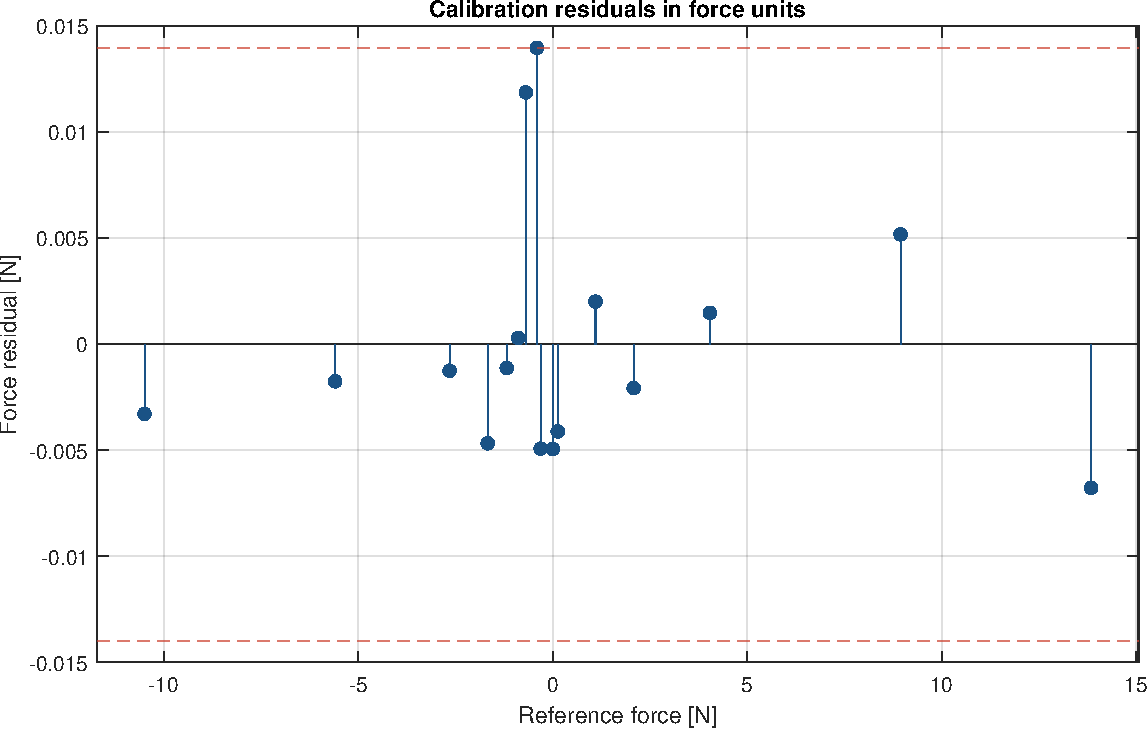
\includegraphics[width=0.76\linewidth]{load_cell_residuals.pdf}
    \caption{Calibration residuals after conversion to force units.}
    \label{fig:calibration-residuals}
\end{figure}

\subsection{Estimator stability}

Figure~\ref{fig:load-stability} reports representative cumulative means. Large reference loads stabilise rapidly because the signal level is high relative to drift and noise. Tests close to zero require longer records; the maximum operational stabilisation time is 25.99~s. This result justifies estimating the calibration voltage from the final $30\%$ rather than from the complete transient record.

\begin{figure}[htbp]
    \centering
    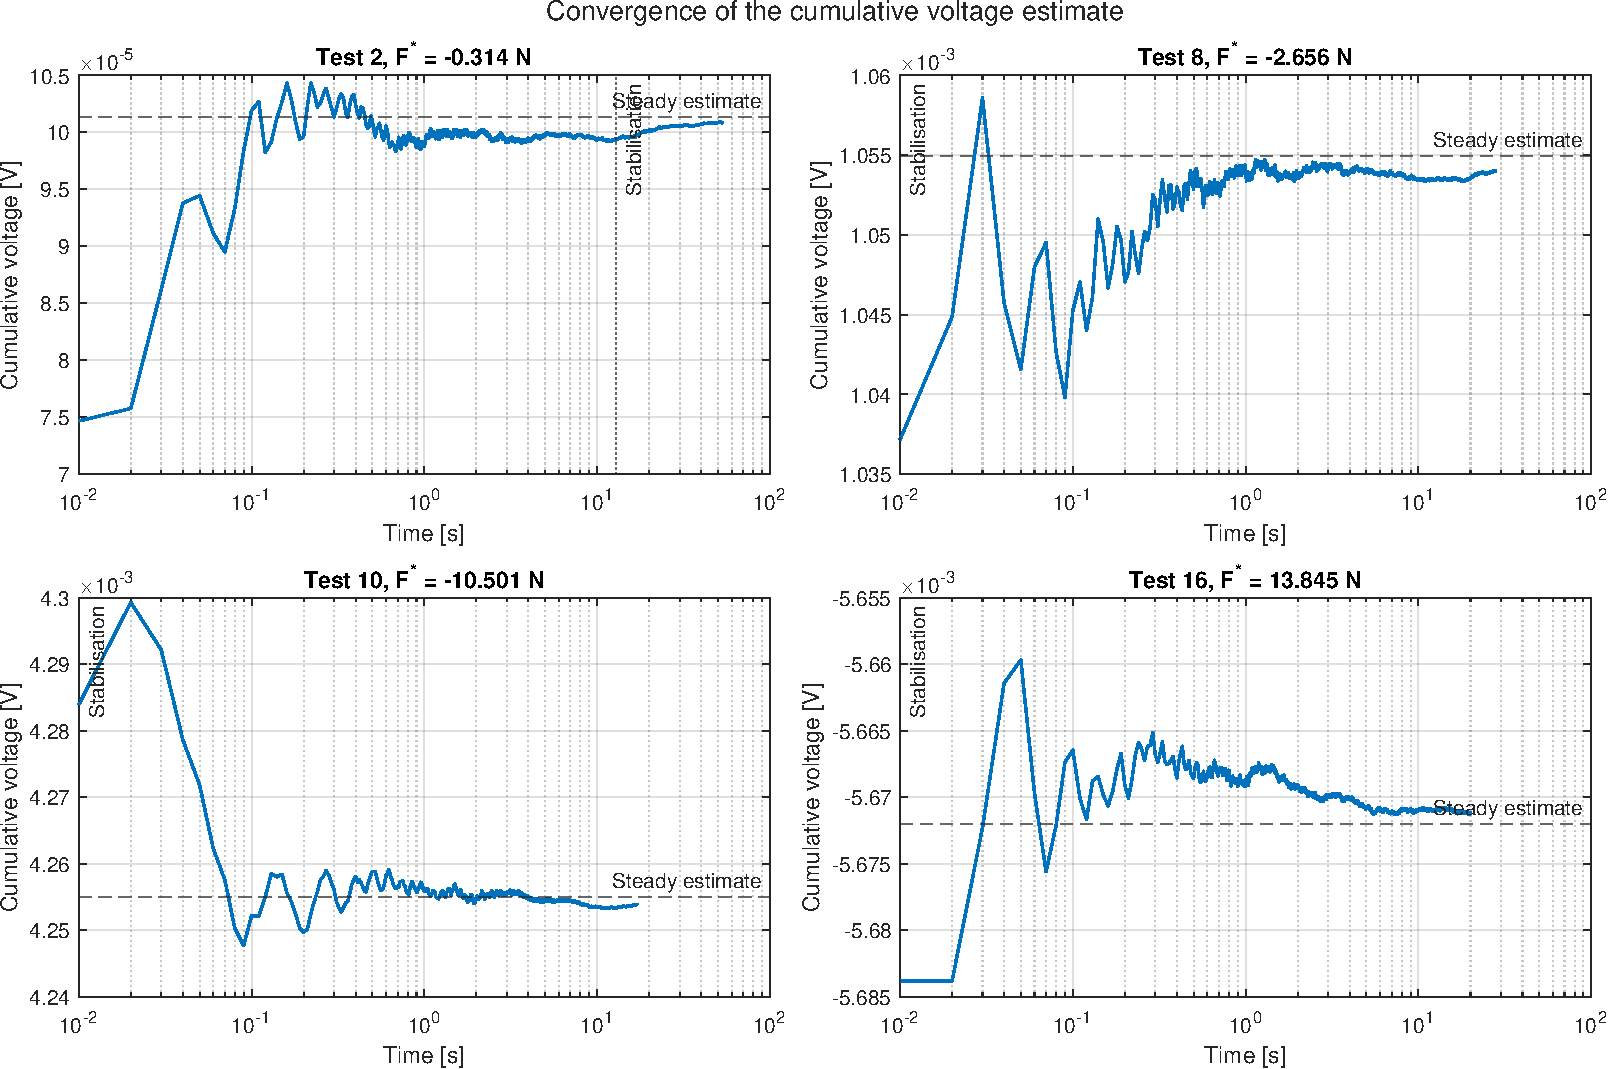
\includegraphics[width=0.94\linewidth]{load_cell_stability.pdf}
    \caption{Convergence of the cumulative voltage estimate for four representative calibration tests.}
    \label{fig:load-stability}
\end{figure}

The calibration therefore supports two distinct statements. The static relation is strongly linear, while near-zero measurements remain sensitive to settling and offset estimation. This distinction is retained when interpreting the mean lift coefficient.

As a check on the influence of individual reference loads, the calibration was refitted sixteen times, omitting one acquisition at a time. The fitted sensitivity changes by less than $0.04\%$ relative to the full-data estimate. This indicates that the transfer-function slope is not controlled by a single load point. The leave-one-out check does not remove the near-zero settling limitation, nor does it constitute an independent validation of the reference masses.

\section{Velocity-field characterisation of the cylinder wake}

\subsection{Mean field}

The time-averaged velocity magnitude and vectors are shown in Figure~\ref{fig:wake-mean}. The cylinder is represented by the masked circular region. Immediately downstream, the streamwise velocity decreases and a wake deficit develops around the centreline. The vectors also show transverse motion associated with the separated shear layers.

\begin{figure}[htbp]
    \centering
    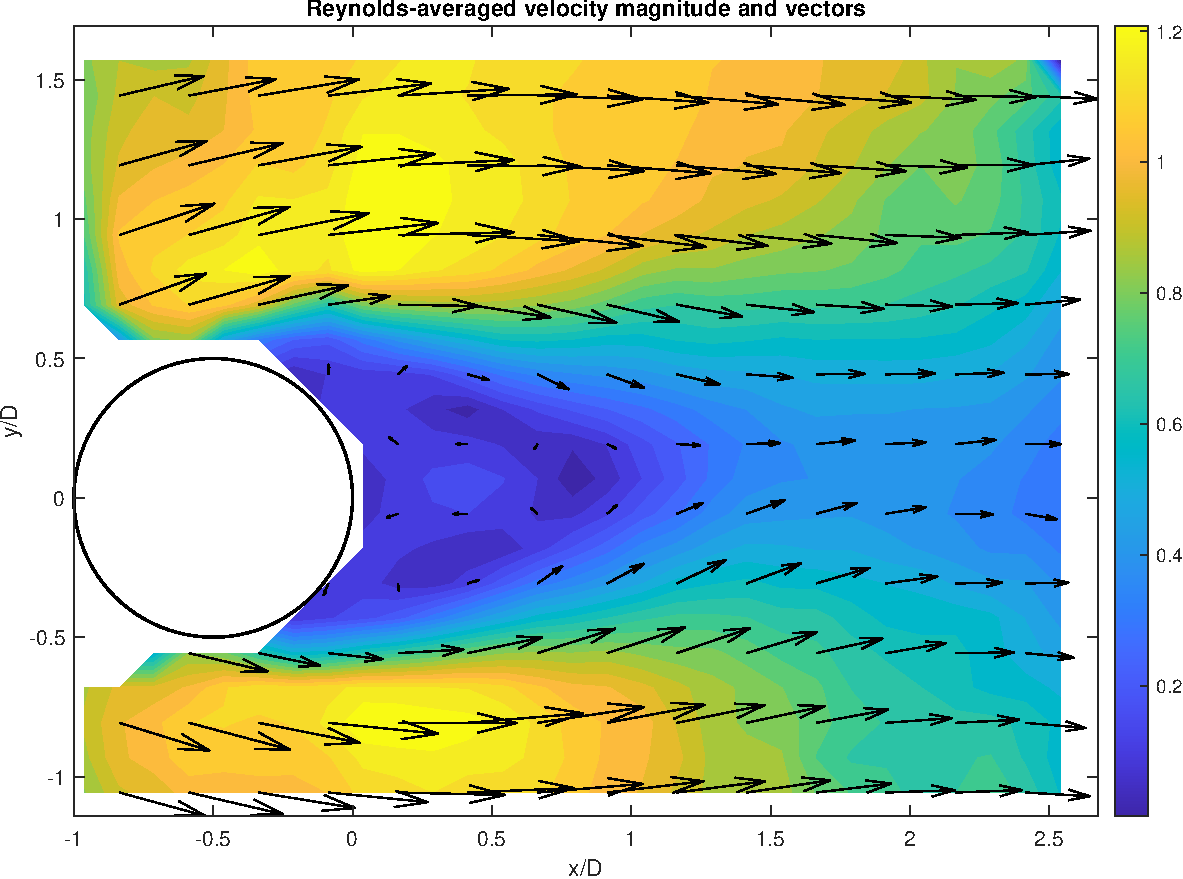
\includegraphics[width=0.88\linewidth]{wake_mean_velocity_field.pdf}
    \caption{Mean dimensionless velocity magnitude and vectors at $Re_D\simeq9980$.}
    \label{fig:wake-mean}
\end{figure}

The field is Reynolds-averaged over the available record. Since the PSV grid contains a substantial fraction of invalid samples near boundaries and regions of weak image correlation, spatial features supported by few valid vectors should not be overinterpreted. No spatial interpolation is used to fill the mean field.

\subsection{Streamwise recovery}

Figure~\ref{fig:wake-profiles} reports vertical profiles at four downstream positions. The near wake exhibits the strongest velocity deficit and the greatest cross-stream variation. The profiles become progressively smoother downstream, indicating momentum redistribution and wake recovery. The limited field of view does not extend far enough to establish a self-similar far-wake regime.

\begin{figure}[htbp]
    \centering
    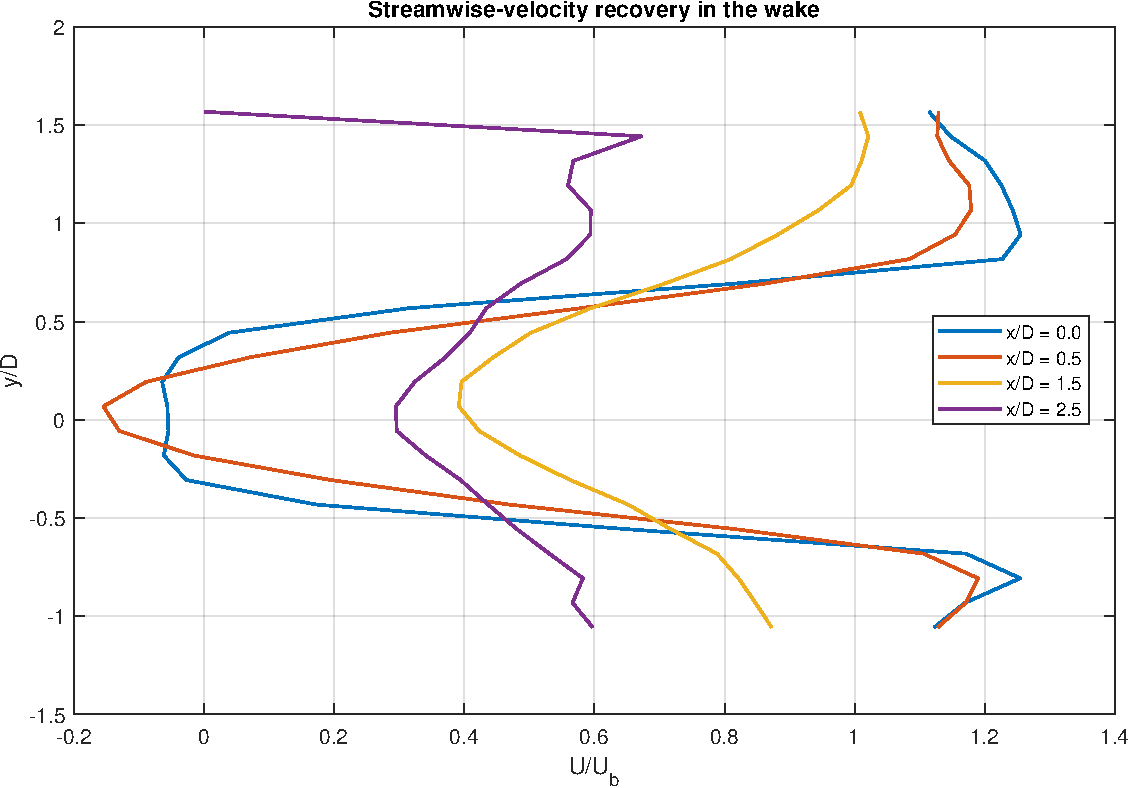
\includegraphics[width=0.74\linewidth]{wake_velocity_profiles.pdf}
    \caption{Recovery of the mean streamwise velocity at selected downstream positions.}
    \label{fig:wake-profiles}
\end{figure}

\subsection{Dominant unsteadiness}

The selected probe is located at $(x/D,y/D)=(0.288,-0.057)$, the nearest valid grid point to the requested centreline position. Figure~\ref{fig:wake-spectrum} shows the transverse-velocity record and its one-sided spectrum. The dominant peak is $f_s=0.567$~Hz, giving
\begin{equation}
St=\frac{f_sD}{U_b}=0.204.
\end{equation}
This value is consistent with the periodic shedding expected behind a circular cylinder at the present Reynolds number, while confinement and the free surface distinguish the setup from an unbounded flow \cite{norberg2003}.

\begin{figure}[htbp]
    \centering
    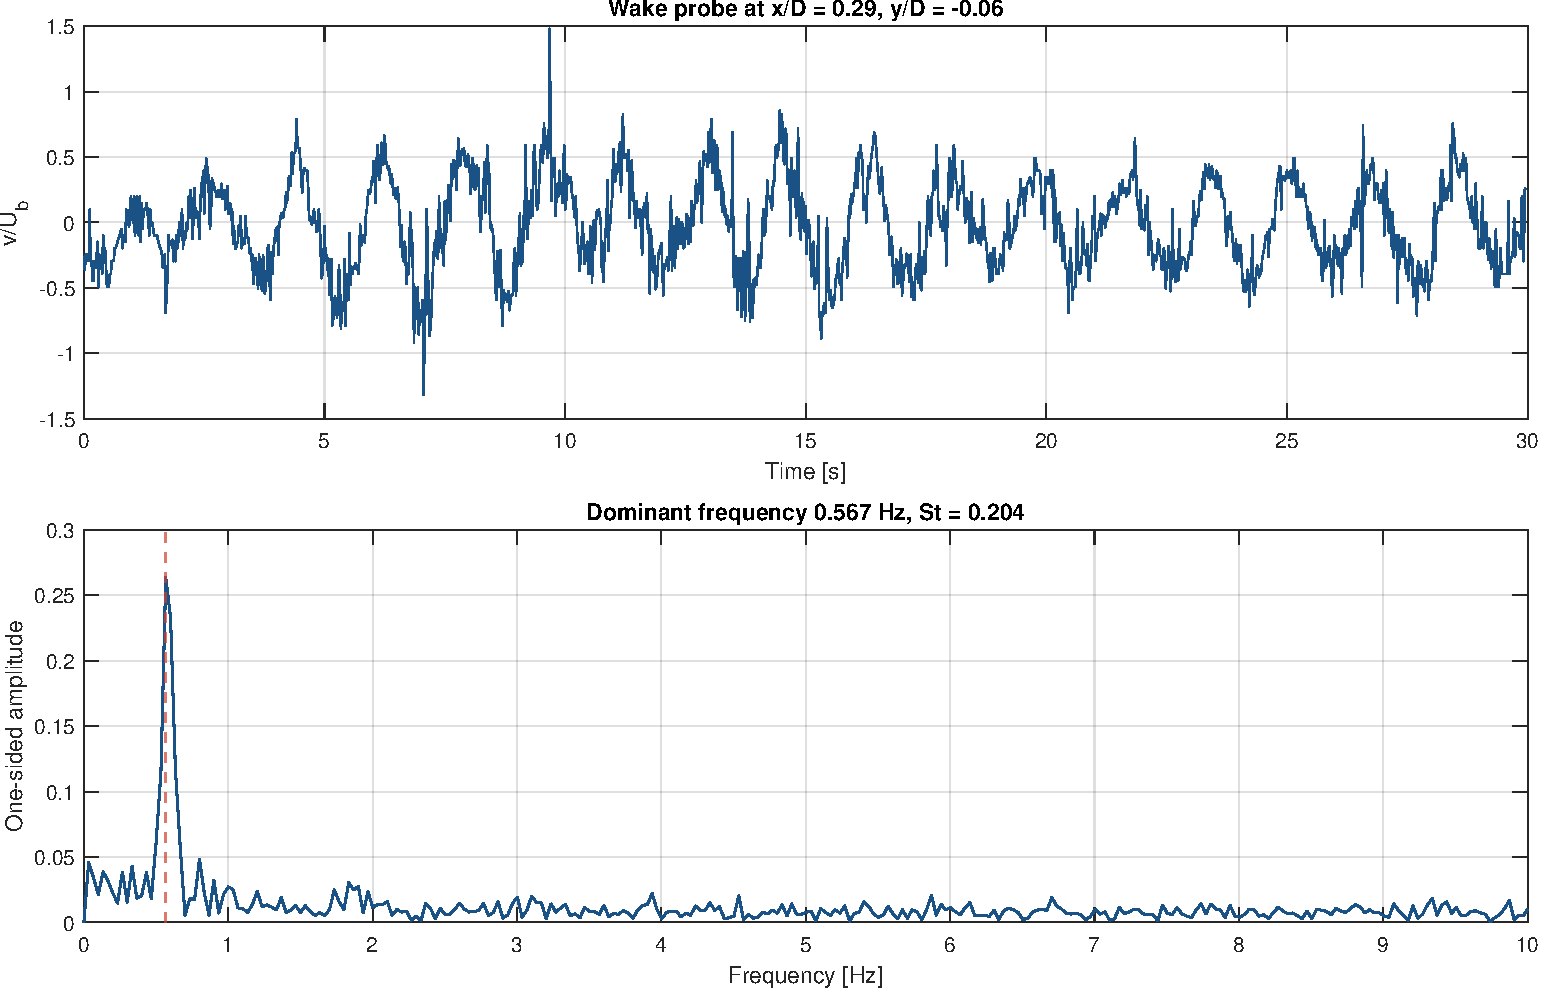
\includegraphics[width=0.88\linewidth]{wake_probe_spectrum.pdf}
    \caption{Transverse velocity at the wake probe and corresponding spectrum.}
    \label{fig:wake-spectrum}
\end{figure}

\subsection{Vorticity sequence}

Figure~\ref{fig:wake-vorticity} presents four frames separated by $90^\circ$ of the identified period. Alternating signed structures form downstream of the cylinder and are convected through the measurement region. The sequence provides a spatial counterpart to the spectral peak: the dominant frequency is associated with an organised alternating wake rather than with isolated measurement noise.

\begin{figure}[htbp]
    \centering
    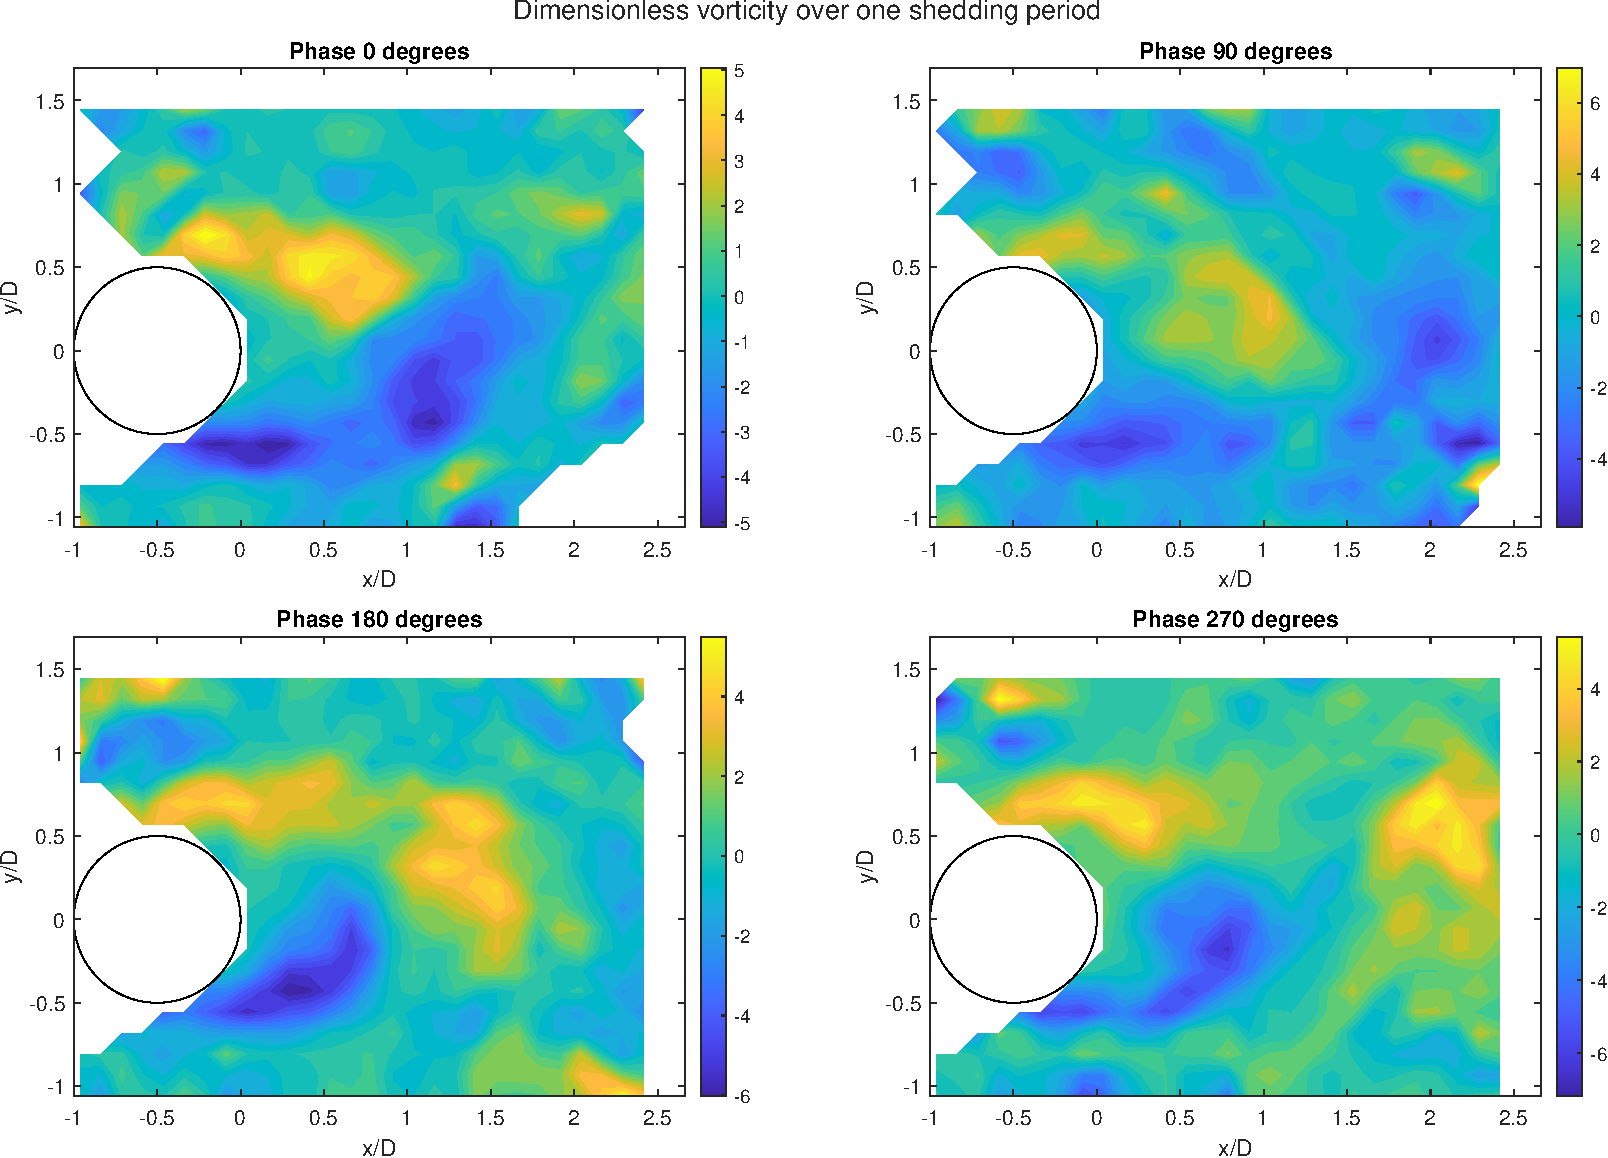
\includegraphics[width=0.93\linewidth]{wake_vorticity_phases.pdf}
    \caption{Dimensionless vorticity at four phases of one shedding period.}
    \label{fig:wake-vorticity}
\end{figure}

The derivative operation amplifies spatial noise, and the frames are not conditional ensemble averages. Consequently, the vorticity sequence is used to identify topology and phase progression, not to report peak vorticity values.

\section{Cylinder-force results}

\subsection{Mean forces}

Figure~\ref{fig:cylinder-forces} shows the measured drag and buoyancy-corrected lift. The mean values are $\overline{F_D}=0.9223$~N and $\overline{F_L}=-0.0172$~N, giving
\begin{equation}
\overline{C_D}=1.4987, \qquad \overline{C_L}=-0.0280.
\end{equation}
The non-zero mean lift is small compared with the drag but cannot be interpreted as evidence of a physical asymmetry by itself. Its magnitude is comparable with the propagated lift uncertainty and remains sensitive to buoyancy subtraction, water-level mismatch, and alignment.

\begin{figure}[htbp]
    \centering
    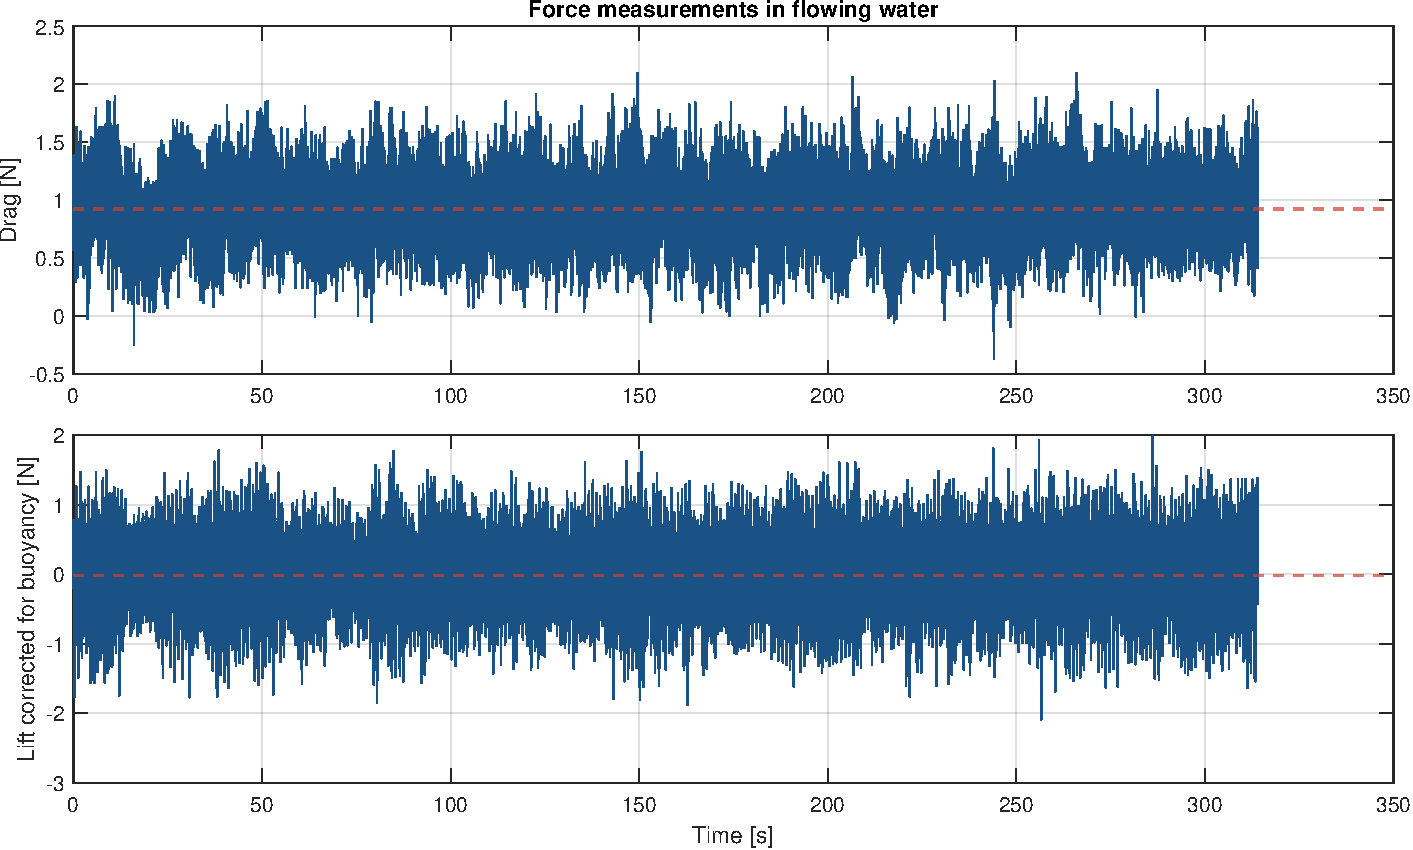
\includegraphics[width=0.88\linewidth]{cylinder_forces.pdf}
    \caption{Drag and buoyancy-corrected lift in flowing water.}
    \label{fig:cylinder-forces}
\end{figure}

\subsection{Force spectrum}

The lift spectrum in Figure~\ref{fig:lift-spectrum} contains a dominant peak at $f_s=1.006$~Hz. With $U_b=0.3333$~m/s and $D=0.06$~m, this gives $St=0.181$. Lift is used because alternating vortex shedding produces a direct cross-stream forcing signature, whereas drag primarily responds at the mean and at even harmonics.

\begin{figure}[htbp]
    \centering
    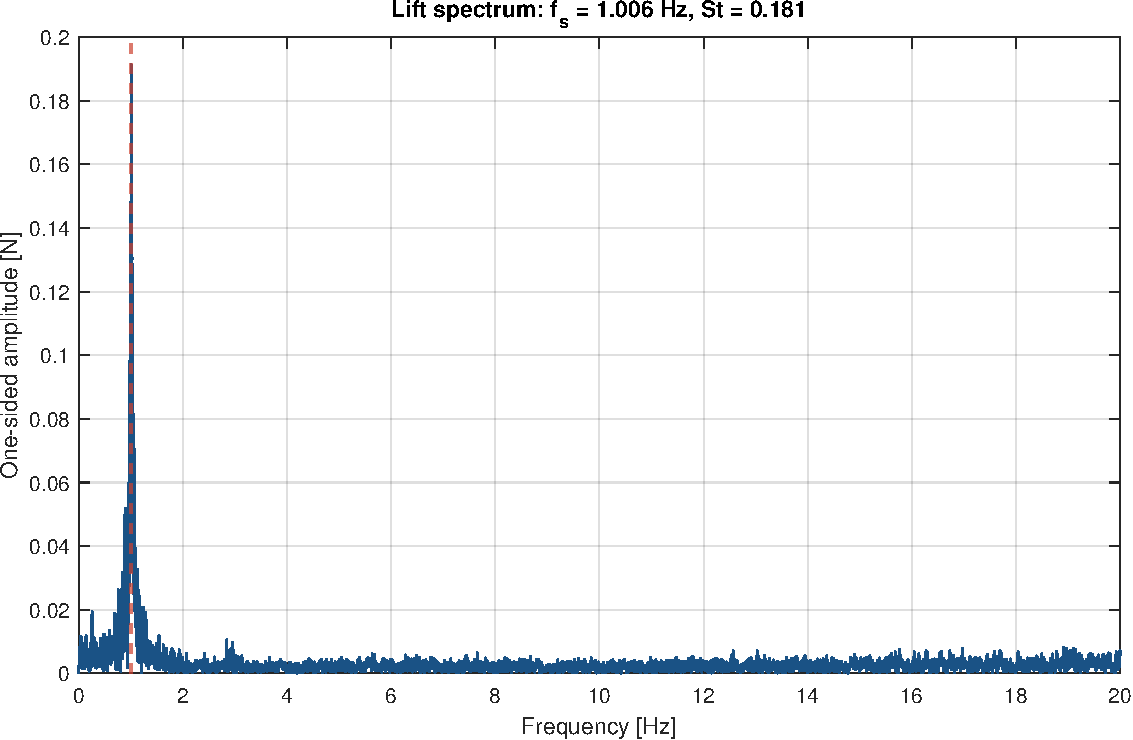
\includegraphics[width=0.74\linewidth]{cylinder_lift_spectrum.pdf}
    \caption{One-sided amplitude spectrum of the corrected lift signal.}
    \label{fig:lift-spectrum}
\end{figure}

The peak is narrow relative to the surrounding spectrum, supporting a coherent periodic component. Its Strouhal number is $11.3\%$ below the PSV estimate, but the two acquisitions have different bulk velocities and water depths. Agreement should therefore be judged at the level of the shedding regime, not as a repeated measurement of a single operating point.

\subsection{Uncertainty budget}

First-order propagation gives standard uncertainties $u(C_D)=0.0756$ and $u(C_L)=0.0574$. The relative standard uncertainty of mean drag is approximately $5.0\%$. For mean lift, a relative percentage is not informative because the measured mean is close to zero. Figure~\ref{fig:force-uncertainty} shows the variance contributions. Force measurement dominates both coefficients; velocity uncertainty is the next relevant contribution to drag because both coefficients scale with $U_b^{-2}$.

\begin{figure}[htbp]
    \centering
    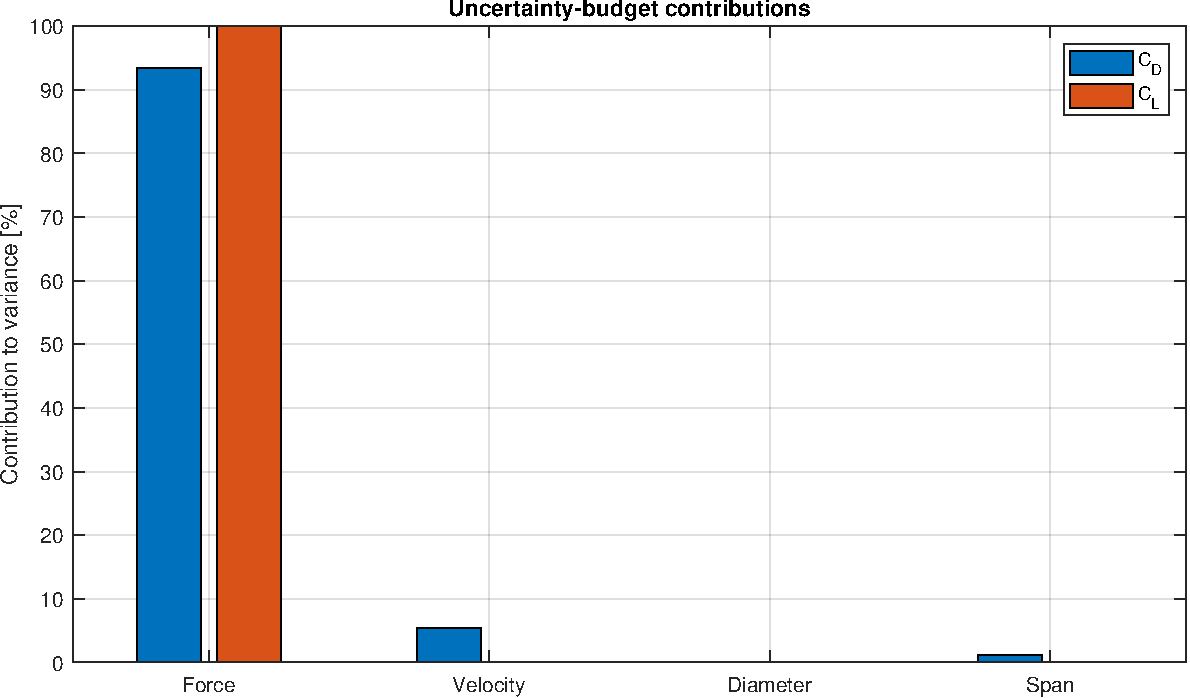
\includegraphics[width=0.80\linewidth]{cylinder_force_uncertainty.pdf}
    \caption{Contributions to the propagated variance of the force coefficients.}
    \label{fig:force-uncertainty}
\end{figure}

A 2~mm mismatch in the water level between the still-water and flow acquisitions would change $C_L$ by approximately 0.0229. This systematic scenario is of the same order as $\overline{C_L}$ and confirms that the present experiment supports a near-zero mean lift rather than a resolved non-zero bias.

\begin{table}[htbp]
\centering
\caption{Principal cylinder results at the two operating conditions.}
\label{tab:cylinder-summary}
\begin{tabular}{lcc}
\toprule
Quantity & PSV acquisition & Force acquisition \\
\midrule
$U_b$ [m/s] & 0.1667 & 0.3333 \\
$Re_D$ & 9980 & --- \\
$f_s$ [Hz] & 0.567 & 1.006 \\
$St$ & 0.204 & 0.181 \\
$\overline{C_D}$ & --- & 1.499 \\
$\overline{C_L}$ & --- & $-0.028$ \\
\bottomrule
\end{tabular}
\end{table}

\section{Synthesis and discussion}

\subsection{What is verified and what is validated}

The laminar case provides the strongest verification statement because both the local velocity profile and the global pressure gradient have analytical references. Their errors, $3.18\%$ and $1.24\%$, are consistent with a correct developed-flow solution and a discretisation error concentrated near the wall. Grid sensitivity below $1\%$ on the final refinement indicates that the remaining discrepancy is not dominated by gross under-resolution.

The turbulent case is a validation problem. No analytical velocity profile exists, and the RANS closure introduces model-form error. The standard $k$--$\varepsilon$ configuration provides the most balanced result for the present data: it has the lowest profile RMSE and a Darcy factor within $0.082\%$ of the experimental reference. The close friction-factor agreement should not be viewed in isolation because integral wall friction can agree even when local profile features differ. Using both metrics reduces that ambiguity.

The low-Reynolds-number closure requires a more cautious reading. Its four-mesh profile differences are non-monotonic, and its turbulence quantities continue to change between the available iteration exports. The friction-factor discrepancy can therefore not be attributed uniquely to closure behaviour or near-wall resolution from the present evidence. The limited spacing-exponent comparison shows small changes in the selected mean profile, but it does not close this verification gap.

The experimental analysis follows the same logic. Calibration establishes traceability from voltage to force before any fluid-mechanics coefficient is evaluated. PSV and force measurements then identify the same physical mechanism through different observables. The velocity field resolves the alternating wake spatially; the lift record resolves its integral loading signature.

For the PSV acquisition, a spatial scan of local spectra recovers the probe Strouhal number at most grid points that satisfy the data-availability criterion. Its peak distribution remains quantised by the finite-record frequency resolution, so the scan is used as a consistency check rather than evidence of a spatially varying shedding frequency. The load-cell slope also remains stable under single-point omission, while this check does not address settling or reference-mass uncertainty.

\subsection{Interpretation of the two Strouhal estimates}

The measured Strouhal numbers are 0.204 from PSV and 0.181 from force data. The absolute difference is 0.023. Three factors prevent treating it as a measurement inconsistency:
\begin{itemize}
    \item the bulk velocity doubles between the two acquisitions;
    \item the water depth changes from 0.42 to 0.45~m;
    \item the estimators use a local transverse velocity and a span-integrated force, respectively.
\end{itemize}
Both values remain representative of periodic circular-cylinder shedding. A stricter cross-validation would require synchronous PSV and force acquisition at the same operating point, with a common clock and documented frequency resolution.

\subsection{Limitations}

The following limitations define the scope of the conclusions:
\begin{itemize}
    \item pairwise grid differences are reported instead of a formal asymptotic GCI;
    \item the turbulent near-wall grid cannot be reconstructed completely from the compact exports;
    \item the uncertainty of the reference pipe-flow profiles is not included in the turbulence-model ranking;
    \item the PSV field contains missing vectors and the phase sequence is not ensemble averaged;
    \item the uncertainty budget is first order and excludes blockage, free-surface deformation, end effects, and alignment;
    \item the cylinder datasets correspond to different operating points and are not synchronous.
\end{itemize}

These restrictions define the range of the conclusions: agreement with the selected benchmarks and consistent identification of the dominant wake dynamics.

\section{Conclusions}

The numerical and experimental analyses provide complementary assessments of canonical internal and separated flows.

For laminar pipe flow, the final refinement changes the selected observables by less than $1\%$. The CFD solution reproduces the developed Poiseuille profile with a relative $L_\infty$ error of $3.18\%$ and the analytical pressure gradient within $1.24\%$. For turbulent pipe flow at $Re_b=75{,}000$, the standard $k$--$\varepsilon$ configuration gives the lowest profile RMSE and a Darcy friction factor of 0.018984, only $0.082\%$ from the experimental reference.

The force transducer is linear over the investigated range, with $R^2=0.9999988$ and a force RMSE of 0.00572~N. Near-zero loads require the longest settling time and define the practical limit for interpreting mean lift. The cylinder experiments give $\overline{C_D}=1.499\pm0.076$ and $\overline{C_L}=-0.028\pm0.057$ as standard-uncertainty results. A local velocity probe gives $St=0.204$, while the lift spectrum gives $St=0.181$ at a second operating condition. Both analyses identify a coherent alternating wake.

The combined results establish a consistent sequence from numerical-resolution assessment and analytical verification to turbulence-model validation, sensor calibration, velocity-field measurement, spectral identification, and uncertainty-aware interpretation.


\begin{thebibliography}{9}
\bibitem{celik2008}
I.~B. Celik, U.~Ghia, P.~J. Roache, C.~J. Freitas, H.~Coleman, and P.~E. Raad,
``Procedure for estimation and reporting of uncertainty due to discretization in CFD applications,''
\emph{Journal of Fluids Engineering}, vol.~130, 078001, 2008.

\bibitem{haaland1983}
S.~E. Haaland,
``Simple and explicit formulas for the friction factor in turbulent pipe flow,''
\emph{Journal of Fluids Engineering}, vol.~105, pp.~89--90, 1983.

\bibitem{launder1974}
B.~E. Launder and D.~B. Spalding,
``The numerical computation of turbulent flows,''
\emph{Computer Methods in Applied Mechanics and Engineering}, vol.~3, no.~2, pp.~269--289, 1974.

\bibitem{norberg2003}
C.~Norberg,
``Fluctuating lift on a circular cylinder: review and new measurements,''
\emph{Journal of Fluids and Structures}, vol.~17, pp.~57--96, 2003.

\bibitem{raffel2018}
M.~Raffel, C.~E. Willert, F.~Scarano, C.~K\"ahler, S.~T. Wereley, and J.~Kompenhans,
\emph{Particle Image Velocimetry: A Practical Guide}, 3rd ed., Springer, 2018.
\end{thebibliography}

\end{document}
